% ------------------------------------------------------------------------
% A Latex "template" for CMP MSc Dissertation
% Produced by Dr. Wenjia Wang through modification of 
% Stanford University PhD thesis style file.  
% 
% Brief Instructions
%#### 
% 1. Write your abstract in a separate tex file and name it as ABS.tex
% 2. Write your acknowledgement in a separate tex file and name it as ACK.tex  
%   Note :  Both ABS and ACK files are already included in the style file. 
% 3. wirte each chapter in a separate tex file and name e.g. Ch1, Ch2, etc. 
% and then use "include" to inlcude them as shown in this example.

% Disclaimer: This template is provided as it is 
% You may use it as you wish, 
% but Dr. Wang won't be resposible for resolving any problems it has or causes.
%
% 
% ------------------------------------------------------------------------
\documentclass[12pt]{report}
\usepackage[centertags]{amsmath}
\usepackage{amsfonts}
\usepackage{amssymb}
\usepackage{amsthm}
\usepackage{newlfont}
\usepackage{graphicx}
\usepackage{tabularx}
\usepackage{array}% http://ctan.org/pkg/array
\usepackage{apalike} % by wjw
\usepackage{pdfsync} %PDF Forward Search
\usepackage{rotating}
\usepackage{subcaption}
\usepackage{url}

\usepackage{CMPDissertation} %CMP Dissertation Style

\usepackage{xtocinc} %Include Table of Contents as the first entry in TOC
%                     Faculty of Grad Studies insists on this!?
%\usepackage[active]{srcltx}  %SRC Specials for DVI search
% Fuzz -------------------------------------------------------------------
\hfuzz2pt % Don't bother to report over-full boxes if over-edge is < 2pt
% Line spacing -----------------------------------------------------------
\newlength{\defbaselineskip}
\setlength{\defbaselineskip}{\baselineskip}
\newcommand{\setlinespacing}[1]%
           {\setlength{\baselineskip}{#1 \defbaselineskip}}
\newcommand{\doublespacing}{\setlength{\baselineskip}%
                           {2.0 \defbaselineskip}}
\newcommand{\singlespacing}{\setlength{\baselineskip}{\defbaselineskip}}
% MATH -------------------------------------------------------------------
\newcommand{\A}{{\cal A}}
\newcommand{\h}{{\cal H}}
\newcommand{\s}{{\cal S}}
\newcommand{\W}{{\cal W}}
\newcommand{\BH}{\mathbf B(\cal H)}
\newcommand{\KH}{\cal  K(\cal H)}
\newcommand{\Real}{\mathbb R}
\newcommand{\Complex}{\mathbb C}
\newcommand{\Field}{\mathbb F}
\newcommand{\RPlus}{[0,\infty)}
%
\newcommand{\norm}[1]{\left\Vert#1\right\Vert}
\newcommand{\essnorm}[1]{\norm{#1}_{\text{\rm\normalshape ess}}}
\newcommand{\abs}[1]{\left\vert#1\right\vert}
\newcommand{\set}[1]{\left\{#1\right\}}
\newcommand{\seq}[1]{\left<#1\right>}
\newcommand{\eps}{\varepsilon}
\newcommand{\To}{\longrightarrow}
\newcommand{\RE}{\operatorname{Re}}
\newcommand{\IM}{\operatorname{Im}}
\newcommand{\Poly}{{\cal{P}}(E)}
\newcommand{\EssD}{{\cal{D}}}
% THEOREMS ---------------------------------------------------------------
\theoremstyle{plain}
\newtheorem{thm}{Theorem}[section]
\newtheorem{cor}[thm]{Corollary}
\newtheorem{lem}[thm]{Lemma}
\newtheorem{prop}[thm]{Proposition}
%
\theoremstyle{definition}
\newtheorem{defn}{Definition}[section]
%
\theoremstyle{remark}
\newtheorem{rem}{Remark}[section]
%
\numberwithin{equation}{section}
\renewcommand{\theequation}{\thesection.\arabic{equation}}
%%% ----------------------------------------------------------------------
\setlength{\tclineskip}{1.05\baselineskip}
%%% ----------------------------------------------------------------------
%\nobib
%\draft
%\nofront

%\permissionfalse

\dedicate{}

%\nolistoftables
%\nolistoffigures

\msc

%\phd
\university{The University of East Anglia}
\school{Computing Sciences}

%#### CHOOSE OR INSERT YOUR MSC COURSE TITLE BELOW #####
% by commentting in your course from the liste befow.

\course{Advanced Computing Science}
%\course{Computing Science}
%\course{Games Development}
%\course{Information Systems}
%\course{Data Mining and Knowledge Discovery}
%\course{Computational Biology}

\copyrightyear{2016}
\submitdate{August 2016}
%\convocation{October}{2012}

% ------------------------------------------------------------------------
% #### Insert the title of your dissertation below.#####
\title{Automated Counting of Wheat Grains in Images}

% #### Insert your full name below.#####
\author{Osagioduwa Edo-Osagie}

%#### insert your supervisor's name below #####
\supervisor{Dr. Wenjia Wang}

%#### insert the name of your markers if you know them #####
\firstmarker{Marker 1: Dr. Wenjia Wang}
\secondmarker{Marker 2: Dr. Ji Zhou}
\examiner{Checker/Moderator}
\organiser{Dr. Wenjia Wang}

% ------------------------------------------------------------------------
\begin{document}
{
\typeout{:?000000000} % Don't bother with over/under-full boxes
\beforepreface
\typeout{:?111111111} % Process All Errors from Here on
}

\afterpreface
\def\baselinestretch{1}
\setlinespacing{1.66}

% ------------------------------------------------------------------------
% ##### Include each chapter in order below #####
% ------------------------------------------------------------------------
% -*-TeX-*- -*-Hard-*- Smart Wrapping
% ------------------------------------------------------------------------
\def\baselinestretch{1}

\chapter{Introduction}

\def\baselinestretch{1.66}


%%% ----------------------------------------------------------------------

% intro text here

\smallskip

%%% ----------------------------------------------------------------------
\goodbreak
\section{Motivation}

\bigskip

%%% ----------------------------------------------------------------------
\goodbreak

\section{Aims and Objectives}




%%% ----------------------------------------------------------------------

% ------------------------------------------------------------------------
% -*-TeX-*- -*-Hard-*- Smart Wrapping
% ------------------------------------------------------------------------
\def\baselinestretch{1}

\chapter{Literature Review and Related Work}

\def\baselinestretch{1.66}


%%% ----------------------------------------------------------------------

% intro text here

\smallskip

%%% ----------------------------------------------------------------------
\goodbreak
\section{The Counting Problem}

\bigskip

%%% ----------------------------------------------------------------------
\goodbreak

\section{Existing Approaches to Counting}
\subsection{Counting by Detection}
\subsection{Counting by Regression}


\bigskip

%%% ----------------------------------------------------------------------
\goodbreak

\section{Learning and Modeling}


\bigskip

%%% ----------------------------------------------------------------------


% ------------------------------------------------------------------------
% -*-TeX-*- -*-Hard-*- Smart Wrapping
% ------------------------------------------------------------------------
\def\baselinestretch{1}

\chapter{Analysis}

\def\baselinestretch{1.66}


%%% ----------------------------------------------------------------------

In this chapter, a critical look is taken at the reviewed literature. Literature concerning the construction of learning models using machine learning was reviewed in the previous chapter, as well as literature concerning different approaches to solving the counting problem. The reviewed methods, techniques and approaches are compared in an attempt to understand how they can be applied to solve our specific problem of counting wheat grains in an image. In addition to this, a closer look is taken at the problem at hand as the data used in the project is described. 

\smallskip

%%% ----------------------------------------------------------------------
\goodbreak
\section{Analysis of Literature Review}
\subsection{Learning and Modeling}
In the literature reviewed, support vector machines (SVMs) and artificial neural networks were predominantly used for learning and modeling tasks when such approaches were taken to solving the counting problem. In particular, SVMs were usually applied to regression tasks, using a slight modification to the traditional SVM algorithm known as \textit{support vector regression}. Neural networks on the other hand, were always applied to classification tasks. Occasionally, ensemble learning was used to improve the results of the classification tasks.\\ \\
%
In some of the more recent literature, it was found that a deep learning approach to learning was taken. In particular, a variation of the artificial neural network known as the \textit{Convolutional Neural Network} (CNN) was applied in most of these works. CNNs differ from traditional neural networks in that the layout of its neurons and layers is inspired by the way the visual cortex works in animals. Because of this, CNNs are suitable for image and video recognition tasks. However, for CNNs to be truly useful, they require several layers which translates to a high computational cost as well as higher technical difficulty in implementation. They also require a high number of images for training. While traditional neural networks (eg. Multi-Layer Perceptron neural networks) also require medium to large size datasets for training, they do not necessarily need to be structured to have many hidden layers. This is a fundamental requirement of deep learning which in some cases, would be more trouble than its worth.

\subsection{Counting}
From the literature reviewed, it can be seen that most approaches to solving the counting problem can be divided into two groups, namely - ``counting by detection'' and ``counting by regression''. Taking a detection approach is more challenging than taking a regression approach as regression approaches sidestep the hard detection problem altogether. However, in addition to yielding a count, detection approaches also offer the bonus of identifying and localizing instances of the subject of the counting problem. Also, the accuracy of regression approaches is limited. This is because these approaches simply aim to estimate some function which can provide a direct mapping from the image to a count, or more truthfully, an estimation of the actual count. It is impossible for one function to provide an exact mapping for all images. Detection methods on the other hand, could theoretically provide \textit{exact} counts from all kinds of images. Of course, this relies completely on such a system being able to accurately detect query instances in images. Difficult to achieve as it might be, it is still possible; even if not perfectly, at least to a very high degree. Of course\\ \\
%
Regression is a supervised learning problem. This means that regression methods will require labeled training data. Also, because regression approaches discard all information concerning the location, nature and features of the objects, using only its 1-dimensional statistics - object count - for learning, a large number of training images will need to be supplied. Keep in mind that counts will need to be supplied with each training image to serve as a label during training. While this may not usually be an issue, in certain scenarios, this might be problematic. This project contains one of such scenarios. The images in question here contain wheat bushes with thousands of grains and a grain count will need to be supplied with each image. The labeling process cannot be automated because the same automated counting is the problem in question. This means that the grains in each of the numerous images will need to be counted by eye which is a very time-consuming and labour intensive task.\\ \\
%
Detection methods however, usually assume a uniformity in the problem space and depend on this assumption. In real-life applications, this may not always be the case. Object detection can be difficult depending on the scenario and detection problem in question. Overlapping instances occluding each other will make detecting and localizing individual instances tricky. Because detection approaches rely completely on the accurate detection of instances, the accuracy of these approaches in such scenarios and problem spaces is \textit{typically} not very high. While counting-by-regression methods cannot really be completely accurate, they are simpler to implement and are less sensitive to non-uniformities in images. Counting-by-detection methods are more powerful and more accurate than counting-by-regression methods but are more difficult to get right. However, when gotten right, and in the right scenario are the much better choice for an approach to solving counting problems. Because of this, a counting-by-detection approach was adopted to solving this problem.
\bigskip

%%% ----------------------------------------------------------------------
\goodbreak
\section{Data Description}
\begin{figure}[ht!]
%\centering
\begin{subfigure}{.5\textwidth}
%  \centering
\includegraphics[width=.9\linewidth,height=.7\linewidth,keepaspectratio]{wheat_1.jpg}
  %\caption{MapleTA Question}
  \label{fig:sub1}
\end{subfigure}%
\begin{subfigure}{.5\textwidth}
%  \centering
 \includegraphics[width=.9\linewidth,height=.7\linewidth,keepaspectratio]{wheat_2.jpg}
  %\caption{MapleTA Gradebook}
  \label{fig:sub2}
\end{subfigure}
\caption{Examples of images from dataset}
\label{fig:test}
\end{figure}
We were provided with 13 high resolution images of a wheat growing plot. The images showed the wheat plants at different stages in their development. The orientation and colour of the wheat stalks different in some of the images. 
The first issue here is that 13 images provides very little data for supervised learning. This makes counting-by-regression approaches unsuitable to this problem. On the other hand, the small size of the dataset made it possible to manually count the grains in each image, essentially providing labels for any approaches that are used with said images as well as targets for evaluation. In the following chapter, we will discuss how the matter of the size of the dataset is dealt with using our proposed approach.






%%% ----------------------------------------------------------------------


% ------------------------------------------------------------------------
% -*-TeX-*- -*-Hard-*- Smart Wrapping
% ------------------------------------------------------------------------

%REF_1 - J.A. Hartigan (1975). Clustering algorithms. John Wiley & Sons, Inc.

%REF_2 - Joblove and Greenberg’s (1978) HSL and HSV

%REF_3 - Charnes, A.; Frome, E. L.; Yu, P. L. (1976). "The Equivalence of Generalized Least Squares and Maximum Likelihood Estimates in the Exponential Family". Journal of the American Statistical Association. 71 (353): 169–171.

\def\baselinestretch{1}

\chapter{Proposed Approach 1: Using a Counting-by-Regression Method}

\def\baselinestretch{1.66}


%%% ----------------------------------------------------------------------

% intro text here
In this dissertation, two methods for counting wheat grains in images are proposed. This chapter presents the first method which takes a counting-by-regression approach. The high-level idea of this method is extremely simple: given $N$ training images with their grain counts provided, the goal was to recover a grain density function $F$ as a real function of pixels in the images. The grain density function learns the relationship between the density of spikelets in areas of the image and provides a mapping between said density and the number of grains in the image. New images could then be provided as input to $F$ and an estimate of the number of grains in the provided image returned as output. The grain density function (which serves as the predictive model) is built by constructing a regression model with the textural features computed from the GLCMs of the images in the dataset. The first step in this approach is the textural feature extraction from the images and the next step involves constructing the regression model. This chapter describes each step in the process.

\bigskip

%%% ----------------------------------------------------------------------
\goodbreak
\section{Textural Feature Extraction}
For the system proposed by this approach, all images involved are dealt with as a representation of their textural features as opposed to dealing with the actual images themselves. Textures are complex visual patterns that have characteristics such as brightness, colour and contrast. Because of this, texture is easily perceived by humans and is believed to be a rich source of visual information. Because it is a rich source of visual information, it can be used as a metric for similarity between images as well as for characterizing images. 
\begin{figure}[ht!]
\centering
\includegraphics[scale=0.3]{glcm_1}
\caption{Plot of GLCM descriptors demonstrating their discriminative power}
\label{fig1}
\end{figure}
This approach makes use of \textit{Gray Level Co-occurrence Matrix} (GLCM) texture analysis. GLCM texture analysis was chosen because descriptors computed from the GLCM are quite discriminative. Figure 4.1 shows a two-dimensional plot of the GLCM features extracted from wheat grain images and wheat stalk images. It can be seen that GLCM descriptors are able to adequately discriminate between grain regions and stalk regions.\\ \\
%
In particular, the GLCM descriptors used to construct the feature vectors are \textit{energy (\textbf{ASM})}, \textit{contrast (\textbf{CON})}, \textit{homogeneity (\textbf{HOM})} and \textit{correlation (\textbf{CORR})}. For each image involved with the system in this approach, its GLCM is computed. Each of the previously mentioned descriptors is computed for an image for when the angle between neighbouring pixels $\theta = 0^\circ$, $\theta = 45^\circ$, $\theta = 90^\circ$ and $\theta = 135^\circ$ and the distance between neighbouring pixels, $d = 0$ to build a 16-dimension feature vector describing the image.

\bigskip
%%% ----------------------------------------------------------------------

%%% ----------------------------------------------------------------------
\goodbreak
\section{Building the Model: Linear Regression Analysis for Count Estimation}
The prediction model is developed by performing linear regression analysis on the set of extracted texture-based features. The model learns the relationship between the textural features of the image and the number of grains in the image. Regression analysis is a classic statistical method, and its basic idea is that given some value $y$ and another value $x$, which is a property of $y$, a function $y = f(x)$ is derived. This function $f$ can then be used to determine the value of $y\prime$ given $x\prime$, where $x\prime$ is a newly encountered value of $x$ and $y\prime$ is its corresponding value of $y$.\\ \\
The proposed framework makes use of a linear regression model with the count as the dependent variable and from each of the 4 texture descriptors in the 16-dimension feature vector, it selects the most important values as independent variables. Recall that for each descriptor (\textit{energy}, \textit{contrast}, \textit{homogeneity} and \textit{correlation}), the value of the descriptor is computed in 4 different spatial arrangements $(d,\theta)$. This gives the values $ASM_{00}$, $ASM_{01}$, $ASM_{11}$, $ASM_{10}$, $CON_{00}$, $CON_{01}$, $CON_{11}$, $CON_{10}$, $HOM_{00}$, $HOM_{01}$, $HOM_{11}$, $HOM_{10}$, $CORR_{00}$, $CORR_{01}$, $CORR_{11}$ and $CORR_{10}$. Before building the regression model, Principal Component Analysis (PCA) is applied to the four values denoting the arrangement of each descriptor to yield one representative value for each texture descriptor giving $ASM\text{'}$, $CON\text{'}$, $HOM\text{'}$ and $CORR\text{'}$. The linear least squares method is used to compute the regression equation, ie. the model \cite{REF27}. The linear regression model is of the form:
\begin{equation}
y = \alpha ASM\text{'} + \beta CON\text{'} + \gamma HOM\text{'} +\delta CORR\text{'}
\end{equation}

where $\alpha$, $\beta$, $\gamma$ and $\delta$ are constants calculated by performing a linear regression analysis on the set of training feature vectors and y is the count of grains in the image. Linear regression is used because it does not seem like too much of a stretch to assume that the relationship between the density of grains in an image is directly proportional to the number of grains in the image. This assumption is validated in the Experiments and Discussions chapter.
\bigskip
%%% ----------------------------------------------------------------------

%%% ----------------------------------------------------------------------
\goodbreak
\section{Counting With the Regression Model}
The only thing needed to count grains in images with this method is the regression equation, more specifically, the estimated coefficients and potentially, the intercepts. This means that the model can be represented in simple terms that are easily readable, understandable and accessible to humans (who aren't necessarily familiar with statistical modeling). It also means that the model can easily be stored and shared once it is computed with little or no cost.\\ \\
%
Given a query image whose grain count is desired, the query image is first converted to a textural representation by extracting its GLCM texture features and forming the feature vector as described in the previous section. PCA is applied to each group of the four descriptors in the 16-element vector to yield one representative value for each texture descriptor giving $ASM\text{'}$, $CON\text{'}$, $HOM\text{'}$ and $CORR\text{'}$. To obtain the grain count, the calculated coefficients (and potentially, intercepts) are substituted into equation 4.2.1 with the descriptor values. The solution of the equation is the estimate of the number of grains in the image. 
\bigskip
%%% ----------------------------------------------------------------------


%%%%%%% APPROACH 2 %%%%%%%%%%%%

\def\baselinestretch{1}

\chapter{Proposed Approach 2: Using a Counting-by-Detection Method}
\def\baselinestretch{1.66}


%%% ----------------------------------------------------------------------

% intro text here
In this dissertation, two methods for counting wheat grains in images are proposed. This chapter presents the second method which takes a counting-by-detection approach. The proposed method makes use of both image analysis and computer vision techniques and machine learning techniques. The detection of grains to be counted is carried out in a supervised learning manner and the image is manipulated using computer vision techniques. The system aims to first detect all instances of grains in a given image, then compute the count as the number of instances detected. Figure 5.1 illustrates the design of the system and its various components. The system first pre-processes images, extracting the regions of interest, then breaks the image into  thousands of sub-images. The sub-images are passed to a classifier which has been trained initially and predicts whether a sub-image contains a grain or not. This chapter proposes a solution to the problem of counting the number of grains in an image. The proposed system is broken down into stages and each stage is described in this chapter.

\smallskip

\begin{figure}[ht!]
\centering
\includegraphics[scale=.4]{Images/design_pipeline}
\caption{Placeholder for diagram showing system overview and components}
\label{fig1}
\end{figure}

\smallskip

%%% ----------------------------------------------------------------------
\goodbreak
\section{Grain Counting Pipeline}
\subsection{Image Pre-processing}
The first step in the grain counting process is to identify and remove all parts of the given images that do not contain grains. The aim of this stage is to reduce the problem space by extracting only the regions of the images that we are concerned with - that is, the spikelets and grains. Region of Interest (ROI) extraction also makes the grain detection and counting process accurate. It removes sky, ground, leaves, and background regions from the image. Otherwise, parts of these regions could be wrongly detected as grains and counted.\\ \\
%
ROI extraction is achieved using \textit{segmentation-based object categorization}. This process applies spectral clustering to an image in order to partition the image into distinct regions, known as clusters, based on their colour. The pixels in a cluster are similar to each other in colour but different from pixels in other clusters. In this project, the \textit{\textbf{k-Means Clustering}}\cite{REF25} algorithm is used to cluster the pixels. Given an image of $n$ pixels ($x_1, x_2, ..., x_n$) in the HSV space \cite{REF26} where each element $x_i$ is a vector made up of that pixels hue, saturation and value, we partition the $n$ pixels into $k$ clusters, $C = \{C_1, C_2, ..., C_k\}$ in order to minimize the distance between every pixel and the mean pixel in each cluster. Mathematically, spectral clustering via kmeans can be denoted as:

\begin{equation}
argmin \sum_{i=1}^{k}\sum_{x\in C_i} ||x - \mu_i||^2
\end{equation}

where $\mu_i$ is the mean HSV pixel vector in cluster $i$\\ \\
%
Figure 5.2 shows an illustration of the ROI process. The original image has spectral clustering applied to it as described above (with $k = 5$), and the result of this is shown in Figure 5.2\_(a). Each cluster is shown with a different colour overlayed over it. From this image, we can select the clusters which contain relevant information (grains) and do away with other clusters. Figure 5.2(b) illustrates this as it shows the resulting image after the red, green and purple clusters are removed. The resulting ROI image still contains all of the useful information (ie. grains), but only little else.
\begin{figure}[ht!]
%\centering
\begin{subfigure}{.5\textwidth}
%  \centering
\includegraphics[width=.9\linewidth,height=.7\linewidth,keepaspectratio]{clusters.png}
  \caption{Image showing cluster memberships}
  \label{fig:sub1}
\end{subfigure}%
\begin{subfigure}{.5\textwidth}
%  \centering
 \includegraphics[width=.9\linewidth,height=.7\linewidth,keepaspectratio]{roi.png}
  \caption{ROI image with useful clusters extracted}
  \label{fig:sub2}
\end{subfigure}
\caption{ROI extraction using spectral clustering}
\label{fig:test}
\end{figure}

\subsection{Sub-image Extraction}
The next step in the grain counting process is to break the extracted ROI image into tiny blocks. These blocks might contain grains or they might contain stalks and leaves that were overlooked in the ROI extraction process. A conceptual summary of the proposed system is that it counts which of these blocks contains a grain, thereby giving a grain count for the whole image. However, it is important to also note that one block might contain more than one grain or even only a portion of a grain. So if the conceptual description is applied, the result would not be very accurate. Strictly speaking, the system only yields an estimate of the grain count. To make this estimate as accurate as possible, the division of the image into blocks has to be done as precisely as possible, with blocks containing grains having either just one grain or a large portion of a grain in them.\\ \\
%
The blocks are extracted using a kernel convolution approach. The convolution matrix (or kernel) is an $M$-by-$N$ matrix containing all $1$s. First the image is transformed to greyscale to simplify the convolution process. Each time the kernel is applied, the result of the convolution, which is the sub-image, is stored in a list. Edges are handled using a ``cropping'' approach. That is, if the kernel cannot completely be placed at an edge, that edge is simply ignored.
\begin{figure}[ht!]
\centering
\includegraphics[scale=0.6]{kernel}
\caption{Pseudocode of sub-image extraction using kernel method}
\label{fig1}
\end{figure}
In our implementation, we use a kernel of size $20$-by-$20$ giving square sub-images of length $20$. This value is ideal because it is large enough to contain one grain. Due to visual perspective issues, grains closer to the background appear smaller. A $20$-by-$20$ kernel is still small enough to contain only one or one and a bit more of a grain scaled down. Also, with a kernel of this size, the cropping edge handling approach is of no negative consequence as it highly unlikely that more than a minuscule number of grains will be in the remainder of the edge (which would be less than $20$ pixels wide).

\subsection{Classification}
This is the main step in the grain counting process. Here, the sub-images extracted from the previous step are classified as either containing a grain or not. In particular, a \textit{\textbf{Multi-Layer Perceptron (MLP)}} neural network is used for the classification. The neural network does not deal directly with the images as a whole, but rather with sub-images. Recall that our dataset contains only $12$ images which would not be anywhere near sufficient to properly train the neural network. However, because the neural network deals with sub-images, 13 images is a lot more than enough to train it. In fact, it can be trained using just one of the images in the dataset. When this one image is selected, it can then be broken down into its sub-images of size $20$-by-$20$. Each image yields $5000$ sub-images on average. This is more than sufficient for training the neural network. Unfortunately, the generated sub-images will still need to be labeled in order to be used for training the neural network. This would be a very time consuming and labour-intensive task. Because of this, only $350$ sub-images were hand selected and labeled. The neural network is then trained on these sub-images. When selecting sub-images to be used for training the neural network, care was taken to keep the training data balanced. That is, the numbers of grain sub-images and non-grain sub-images were fairly close. No one class dominated the selected sample.\\ \\
%
It is worth noting that the whole sub-image is not passed into the neural network. Instead, discriminative features are extracted from the sub-images to form feature vectors. We make use of textural features based on the textures of the sub-images. Generally speaking, textures are complex visual patterns that have characteristics such as brightness, colour and contrast. Because of this, texture is easily perceived by humans and is believed to be a rich source of
visual information. For each sub-image, the \textit{Gray Level Co-occurrence Matrix (GLCM)} is computed. From the GLCM, we then compute the following texture descriptors - \textit{energy}, \textit{homogeneity}, \textit{correlation} and \textit{dissimilarity}. Each of these descriptors is computed for when the angle between neighbouring pixels, $\theta = 0^\circ, \theta = 45^\circ, \theta = 90^\circ$ and $\theta = 135^\circ$ and the distance between neighbouring pixels, $d = 0$ to build a 16-dimension feature vector describing the sub-image. This means that 16-element vectors are passed through the neural network, as opposed to $20$-by-$20$ matrices (400-element vectors). This saves memory and also allows the neural network to work faster as well. Figure 4.1 shows GLCM descriptors extracted from different parts of a wheat image and plotted against each other. From the figure, it can be seen that GLCM descriptors are able to adequately discriminate between grain regions and stalk regions. By using GLCM feature vectors instead of raw image data, we can boost the discriminative power of the neural network and improve the accuracy of the detection system.

\subsection{Employing the System to Counting}
Once the neural network is built, it can then be used for the detection of grains. Given a query image, it is passed through the pipeline. First, the query image goes through pre-processing to have the ROI extracted from it. The query ROI image is then broken into query sub-images. Next is the detection stage - the neural network is applied to the query sub-images to determine whether a given sub-image contains a grain or not. The number of sub-images classified as containing grains by the neural network is then returned as an estimate of the number of grains in the image.
\bigskip

%%% ----------------------------------------------------------------------
\goodbreak




\bigskip

%%% ----------------------------------------------------------------------



% ------------------------------------------------------------------------
% -*-TeX-*- -*-Hard-*- Smart Wrapping
% ------------------------------------------------------------------------

% REF\_1 - http://neuralnetworksanddeeplearning.com/chap1.html

% REF\_2 - Large-Scale Machine Learning with Stochastic Gradient Descent Leon Bottou

% REF\_3 - Chin-Wei Hsu, Chih-Chung Chang and Chih-Jen Lin (2010). A practical guide to support vector classification. Technical Report, National Taiwan University.


\def\baselinestretch{1}

\chapter{Experimentation and Discussion}

%%% ----------------------------------------------------------------------

% intro text here

\smallskip

%%% ----------------------------------------------------------------------
\goodbreak

\section{Evaluating the Counting-by-Regression Approach}
\subsection{Evaluation Methodology}
%describe ways used to evaluate - https://en.wikipedia.org/wiki/Regression_validation

\subsection{System Performance}
%experiments and results and discuss

\section{Evaluating the Counting-by-Detection Approach}
\subsection{The Model Setup}
The model used for the prediction (and in essence, detection) of grains was the artificial neural network using the Multi-Layer Perceptron (MLP) learning algorithm. The MLP made use of the \textit{\textbf{sigmoid function $\sigma$}} (also known as the \textbf{\textit{logistic function}}) as its activation function (REF\_1). The sigmoid function is as follows:
\begin{equation}
\sigma(x) = \frac{1}{1 + e^{-x}}
\end{equation}
The MLP used the \textit{\textbf{stochastic gradient descent}} algorithm for tuning its weights (REF\_2). Neural network possess a number of \textit{hyperparameters} which cannot be learned by fitting the model to the data but could influence their performance greatly. In particular, the MLP neural network used for this task had the following hyperparameters:
\begin{itemize}
\item \textit{hidden layer arrangement} - This refers to the number of hidden layers in the network as well as the number of neurons in each layer.
\item \textit{alpha} - This is the \textit{L2} regularization penalty for minimizing prediction error
\item \textit{learning rate} - This controls how quickly the gradient descent algorithm travels down the slope to find the minimum of the cost function when tuning the weights of the neurons.
\item \textit{batch size} - This refers to the size of the mini-batches chosen by the stochastic gradient descent algorithm to speed up the learning process
\end{itemize}
In order to get the best performance from the MLP, an attempt was made to determine the optimum values for these hyperparameters. To do this, the \textit{\textbf{Grid Search}} algorithm for hyperparameter optimization was employed. Grid search is simply an exhaustive search through a manually specified subset of the hyperparameter space (REF\_3).

\subsection{Evaluation Methodology}
350 images were hand selected and labeled to form a data set. The images were selected in a balanced manner with roughly the same amount of instances of all classes. All of this data was used for training and building the neural network. The same data was also used in evaluating the performance of the neural network. Things were done this way because while there was no shortage of sub-images, they had to be labeled manually. Labeling more sub-images for testing than the 350 images already labeled would have been a time-consuming process. On the other hand, we thought it would have been unwise to split the data into separate training and testing sets as the dataset was not very large to begin with. To overcome this problem, \textit{cross validation} was used for evaluation.\\ \\
%
Cross validation aims to define a dataset to ``test'' a model in the training phase, in order to limit problems like overfitting and give an idea of how the model will generalize to an independent dataset. For evaluating the accuracy of our MLP classifier, 5-fold cross validation was used. The data was split into five sets and five iterations of the following procedure were carried out. At each iteration, one set was selected to be the training set (used to build the classifier) and the remaining four were used to test the classifier. The set selected as the training set was changed at each of the five iterations. Once all the iterations were completed, the accuracies from each one was averaged to give the mean accuracy of the classifier. This was needed to get as good a classifier as possible. This is because MLP neural networks start with random weights assigned to the neurons. The values of these starting weights affect the weights that the MLP ends up with, thereby affecting its performance. To get the best model possible, the neural network was built (with random weights) $n$ times. After each build, it was evaluated using the 5-fold cross validation strategy to paint a picture of its accuracy. The MLP with the best accuracy (found to be $81.12\%$) was selected and serialized to disk to be used as the model as needed.


\bigskip

%%% ----------------------------------------------------------------------
\goodbreak

\subsection{System Performance}
\begin{table}[hp!]
  \centering
  \begin{tabular}{ | c | c | c | c |}
    \hline
    Image & Actual count & Predicted count & Time taken \\ \hline
    \begin{minipage}{.3\textwidth}
      \begin{center}
		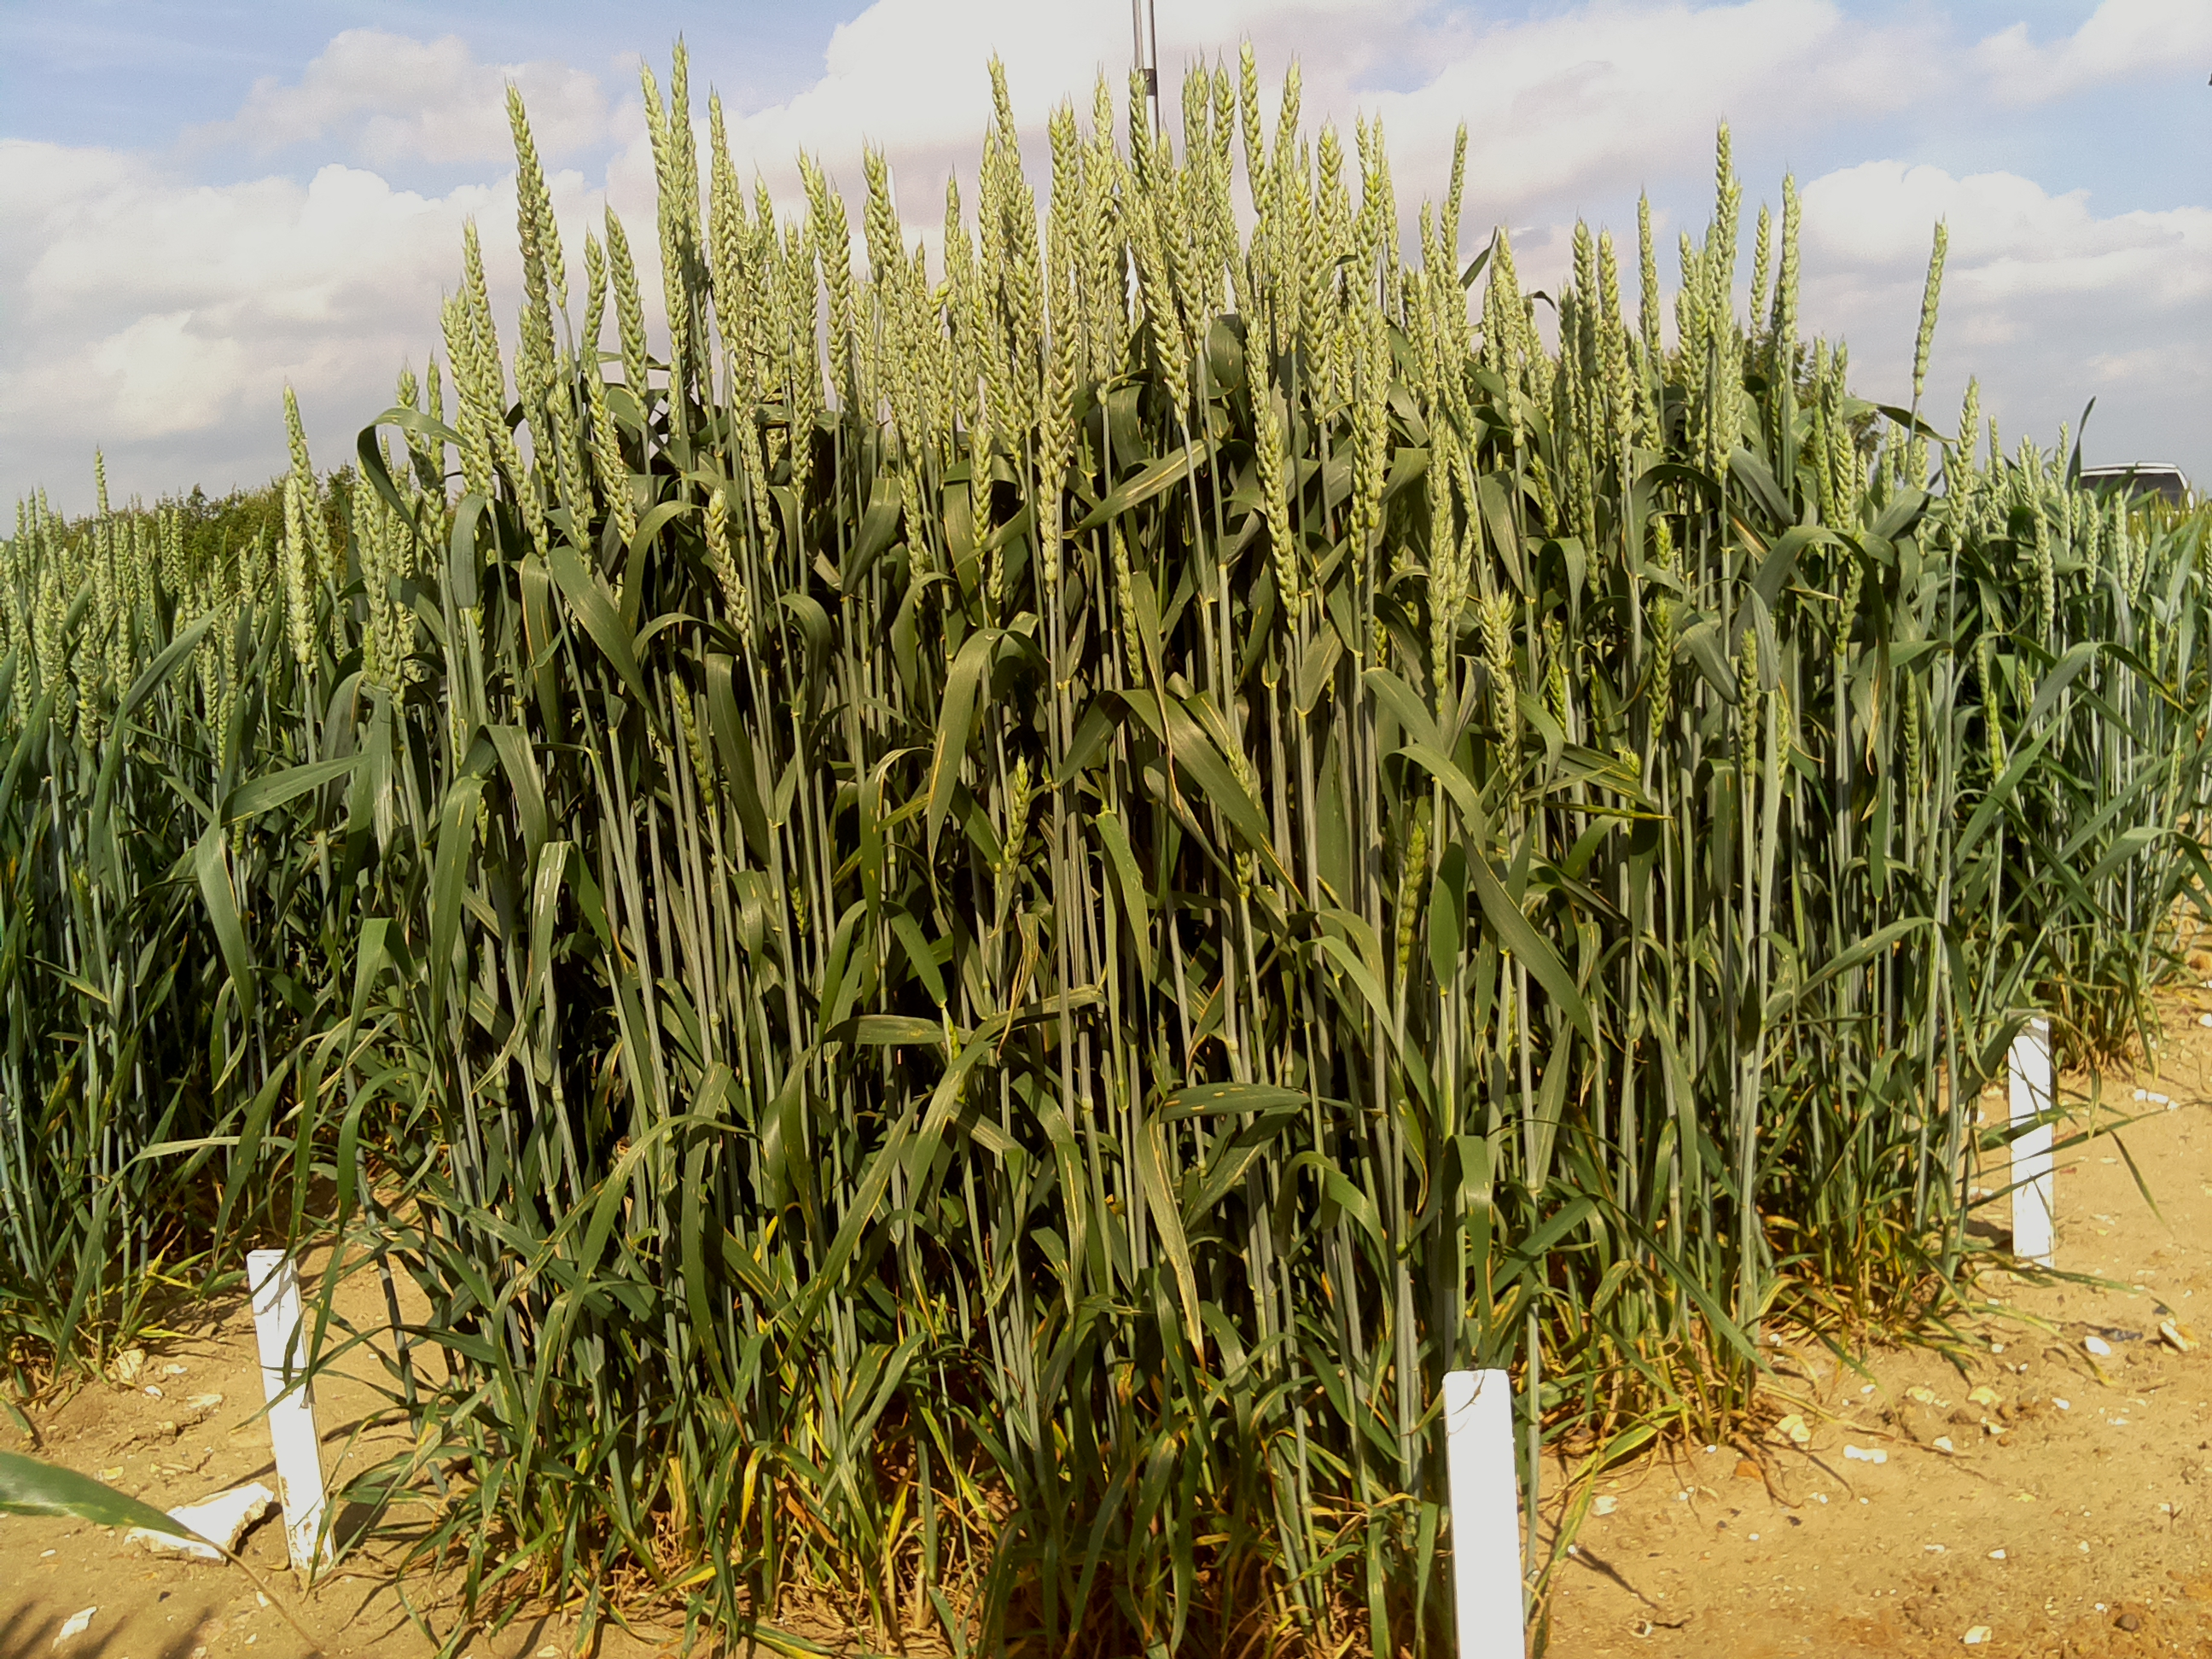
\includegraphics[width=\linewidth]{Images/001}
      \end{center}
    \end{minipage}
    &
    %\begin{minipage}[t]{5cm}
      xxx
    %\end{minipage}
    & 
    %\begin{minipage}{5cm}
      1435
    %\end{minipage}
    & 
    %\begin{minipage}{5cm}
      215
    %\end{minipage}
    \\ \hline
    %%% NEW LINE %%%
    \begin{minipage}{.3\textwidth}
      \begin{center}
		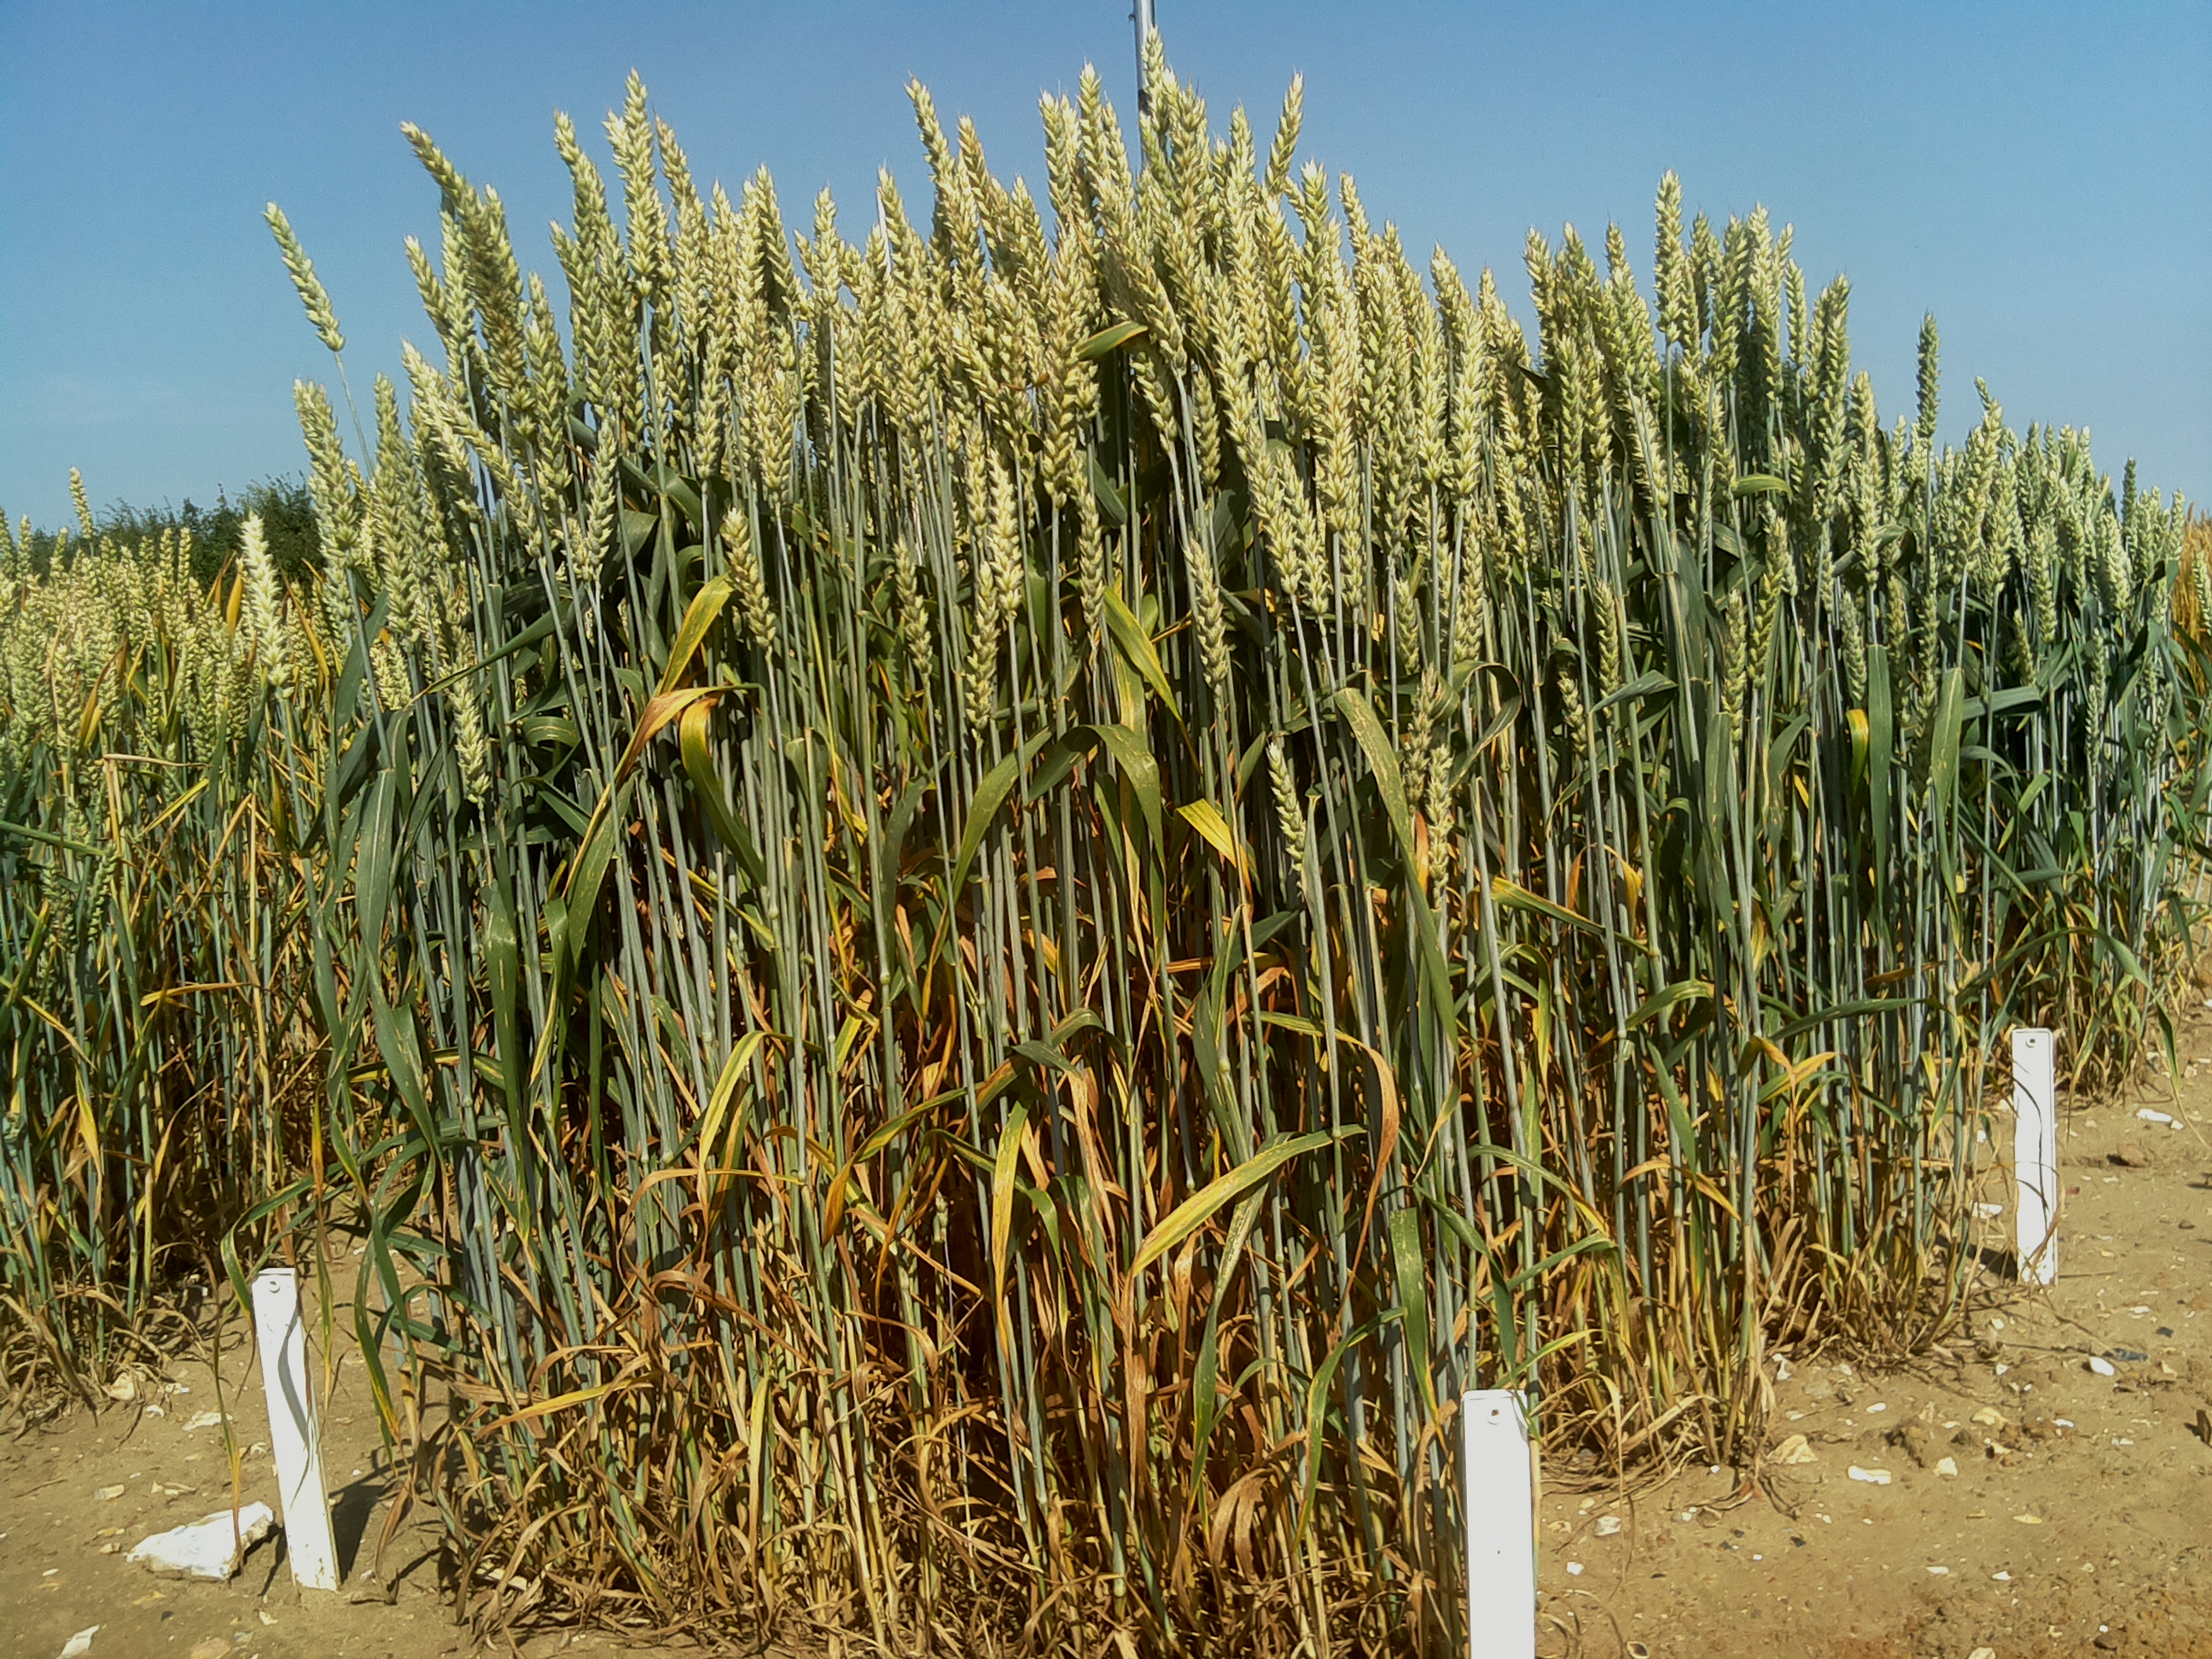
\includegraphics[width=\linewidth]{Images/002}
      \end{center}
    \end{minipage}
    &
    %\begin{minipage}[t]{5cm}
      xxx
    %\end{minipage}
    & 
    %\begin{minipage}{5cm}
      yyy
    %\end{minipage}
    & 
    %\begin{minipage}{5cm}
      zzz
    %\end{minipage}
    \\ \hline
    %%% NEW LINE %%%
    \begin{minipage}{.3\textwidth}
      \begin{center}
		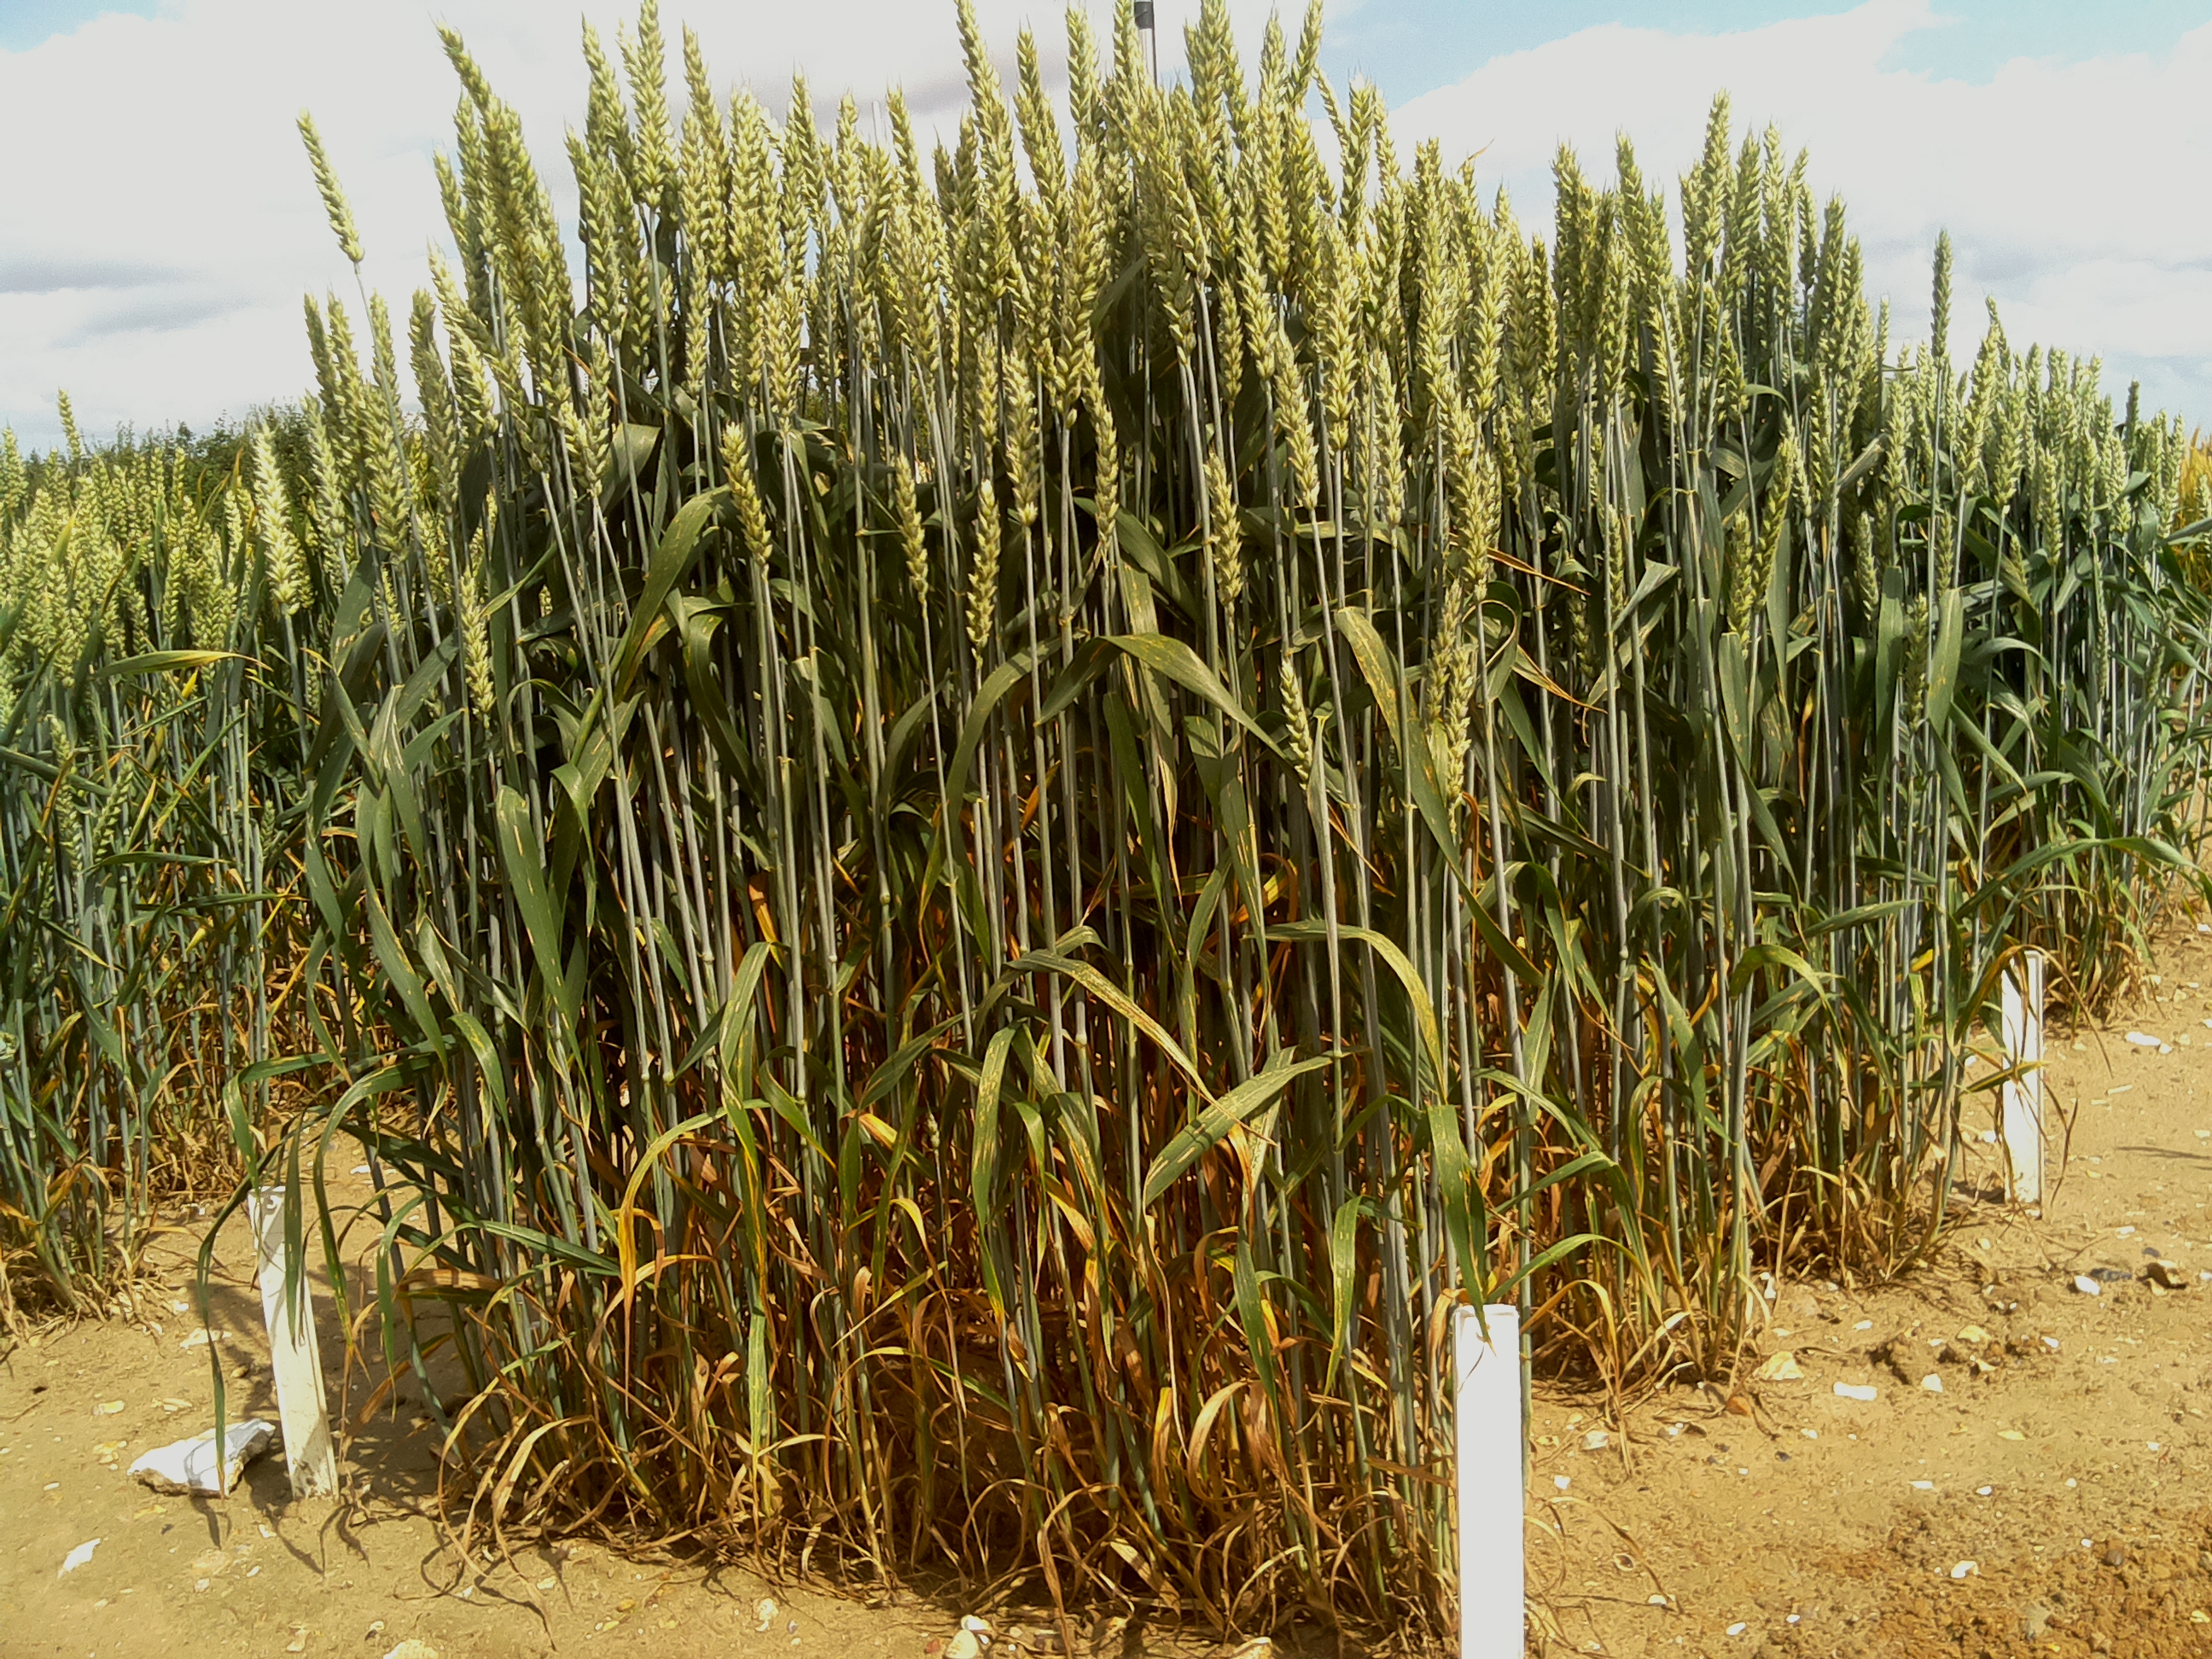
\includegraphics[width=\linewidth]{Images/003}
      \end{center}
    \end{minipage}
    &
    %\begin{minipage}[t]{5cm}
      xxx
    %\end{minipage}
    & 
    %\begin{minipage}{5cm}
      yyy
    %\end{minipage}
    & 
    %\begin{minipage}{5cm}
      zzz
    %\end{minipage}
    \\ \hline
    %%% NEW LINE %%%
    \begin{minipage}{.3\textwidth}
      \begin{center}
		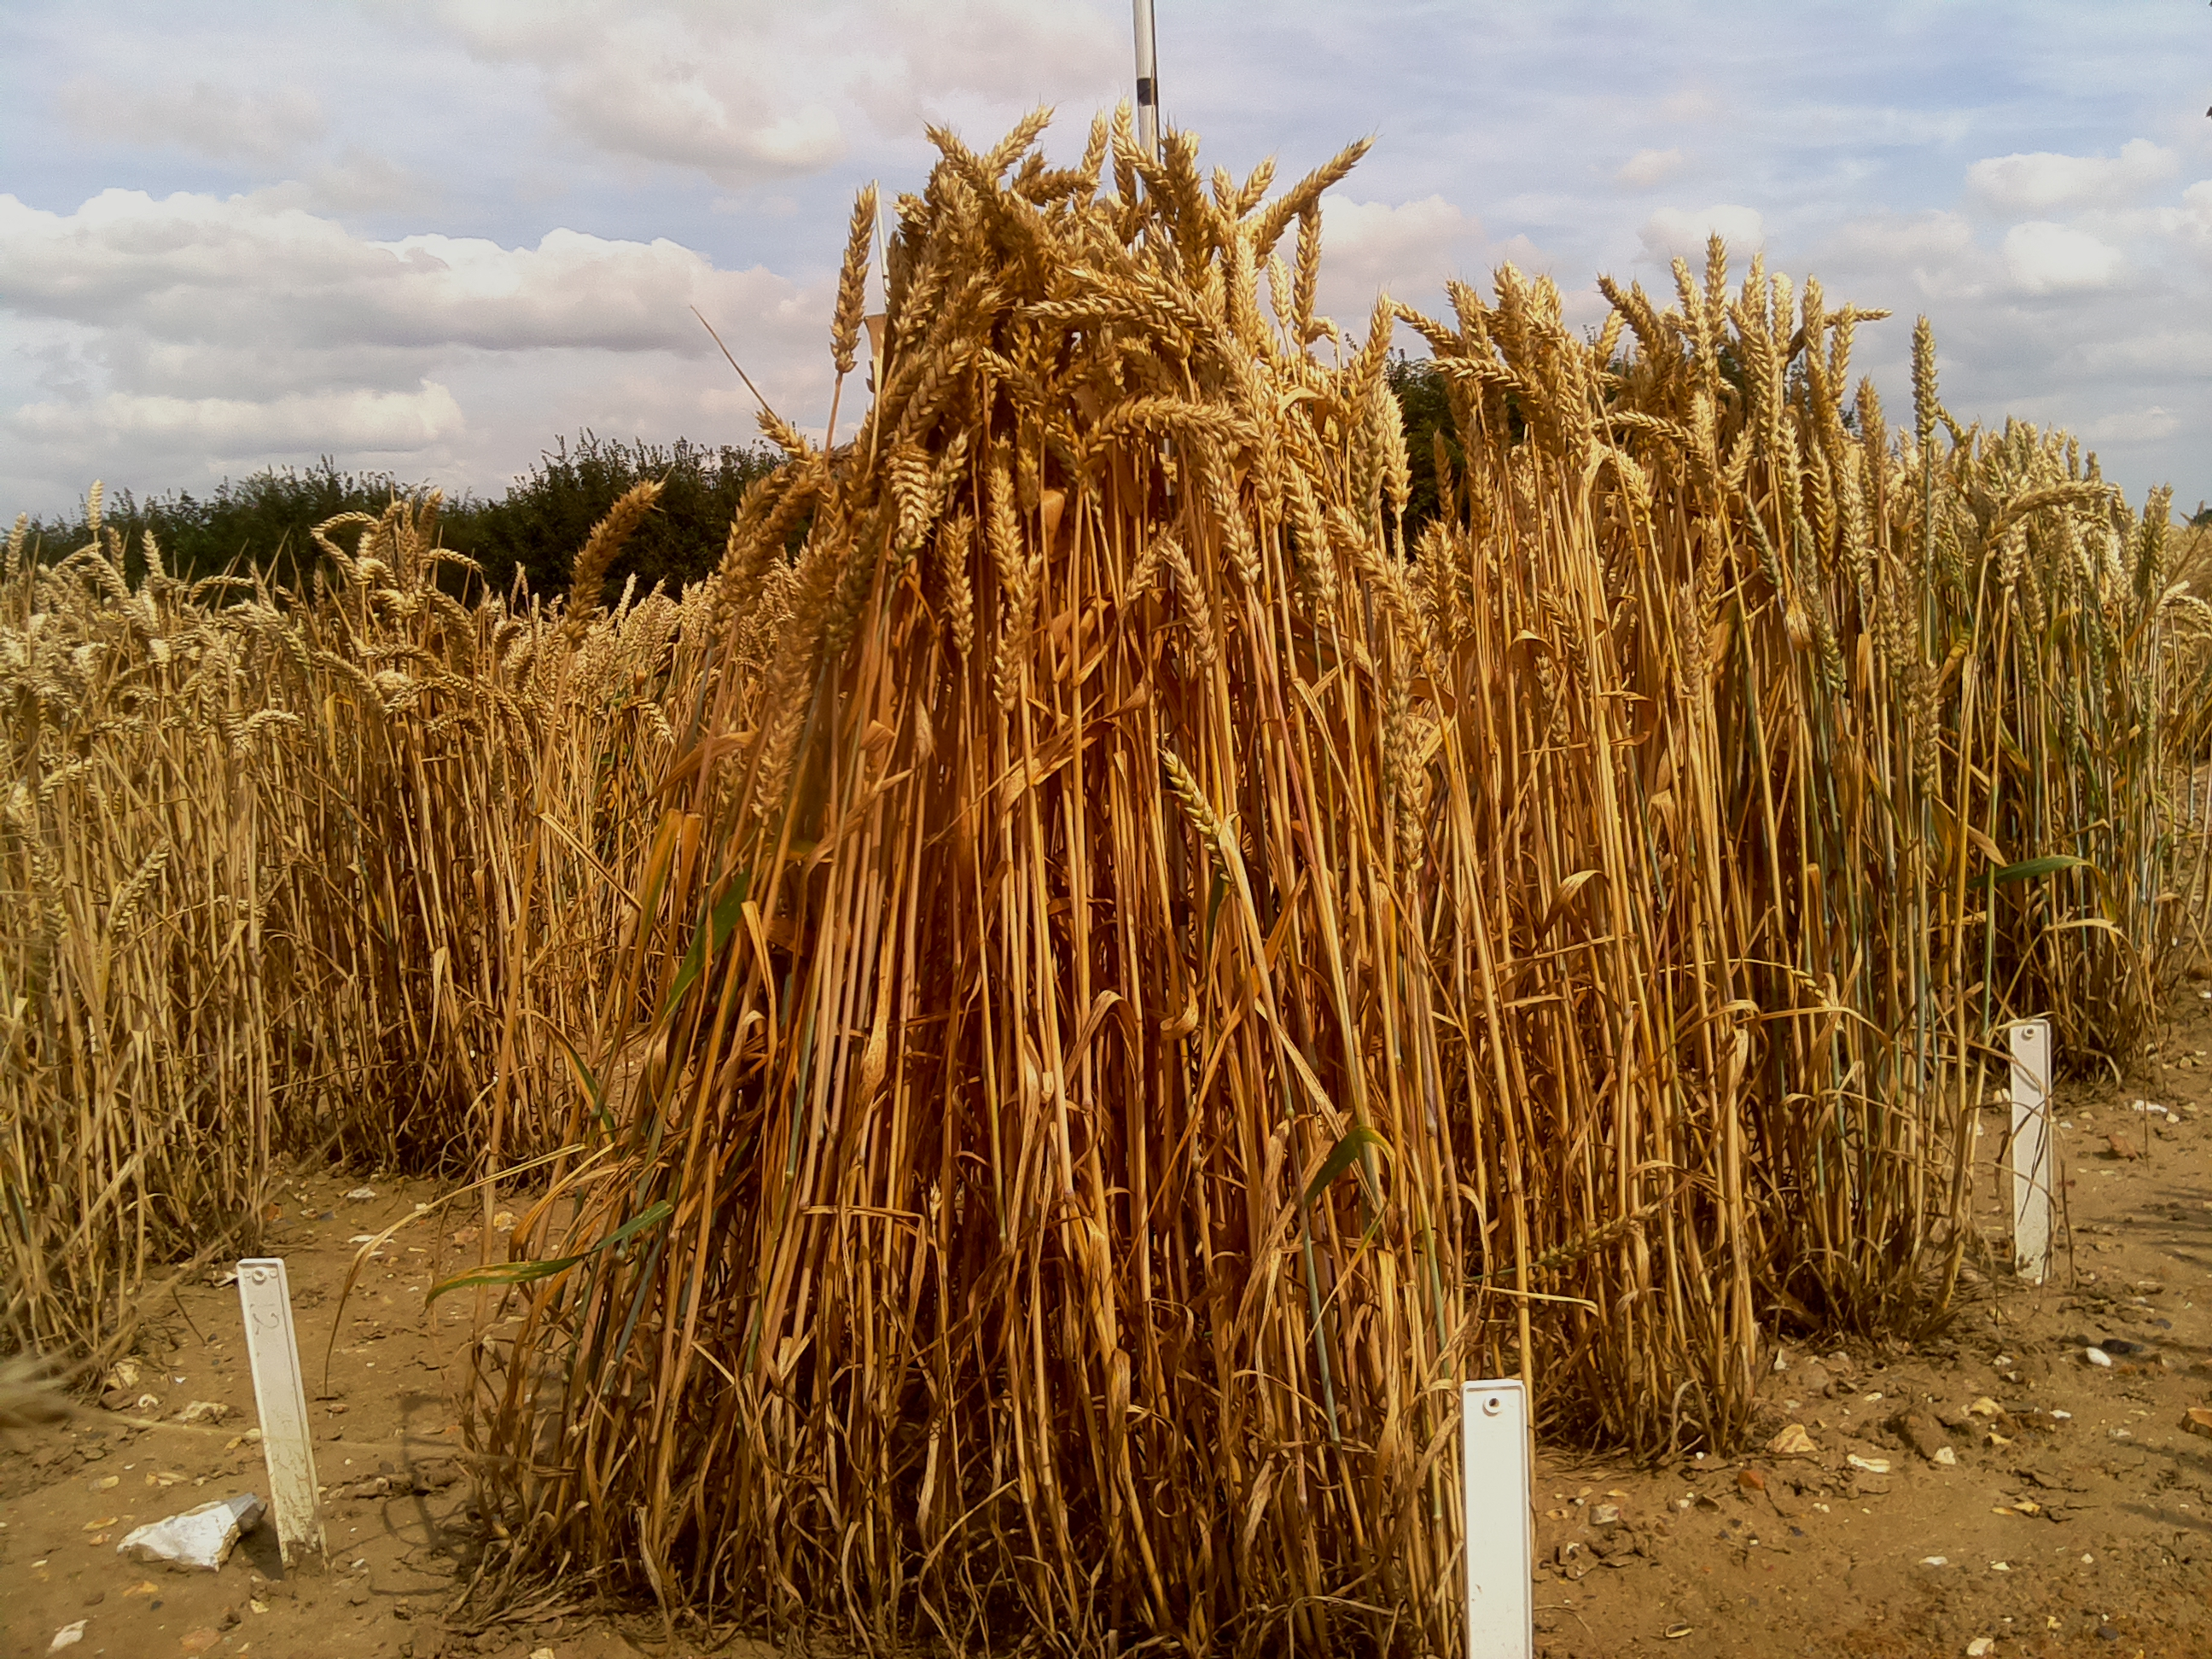
\includegraphics[width=\linewidth]{Images/004}
      \end{center}
    \end{minipage}
    &
    %\begin{minipage}[t]{5cm}
      xxx
    %\end{minipage}
    & 
    %\begin{minipage}{5cm}
      yyy
    %\end{minipage}
    & 
    %\begin{minipage}{5cm}
      zzz
    %\end{minipage}
    \\ \hline
    %%% NEW LINE %%%
    \begin{minipage}{.3\textwidth}
      \begin{center}
		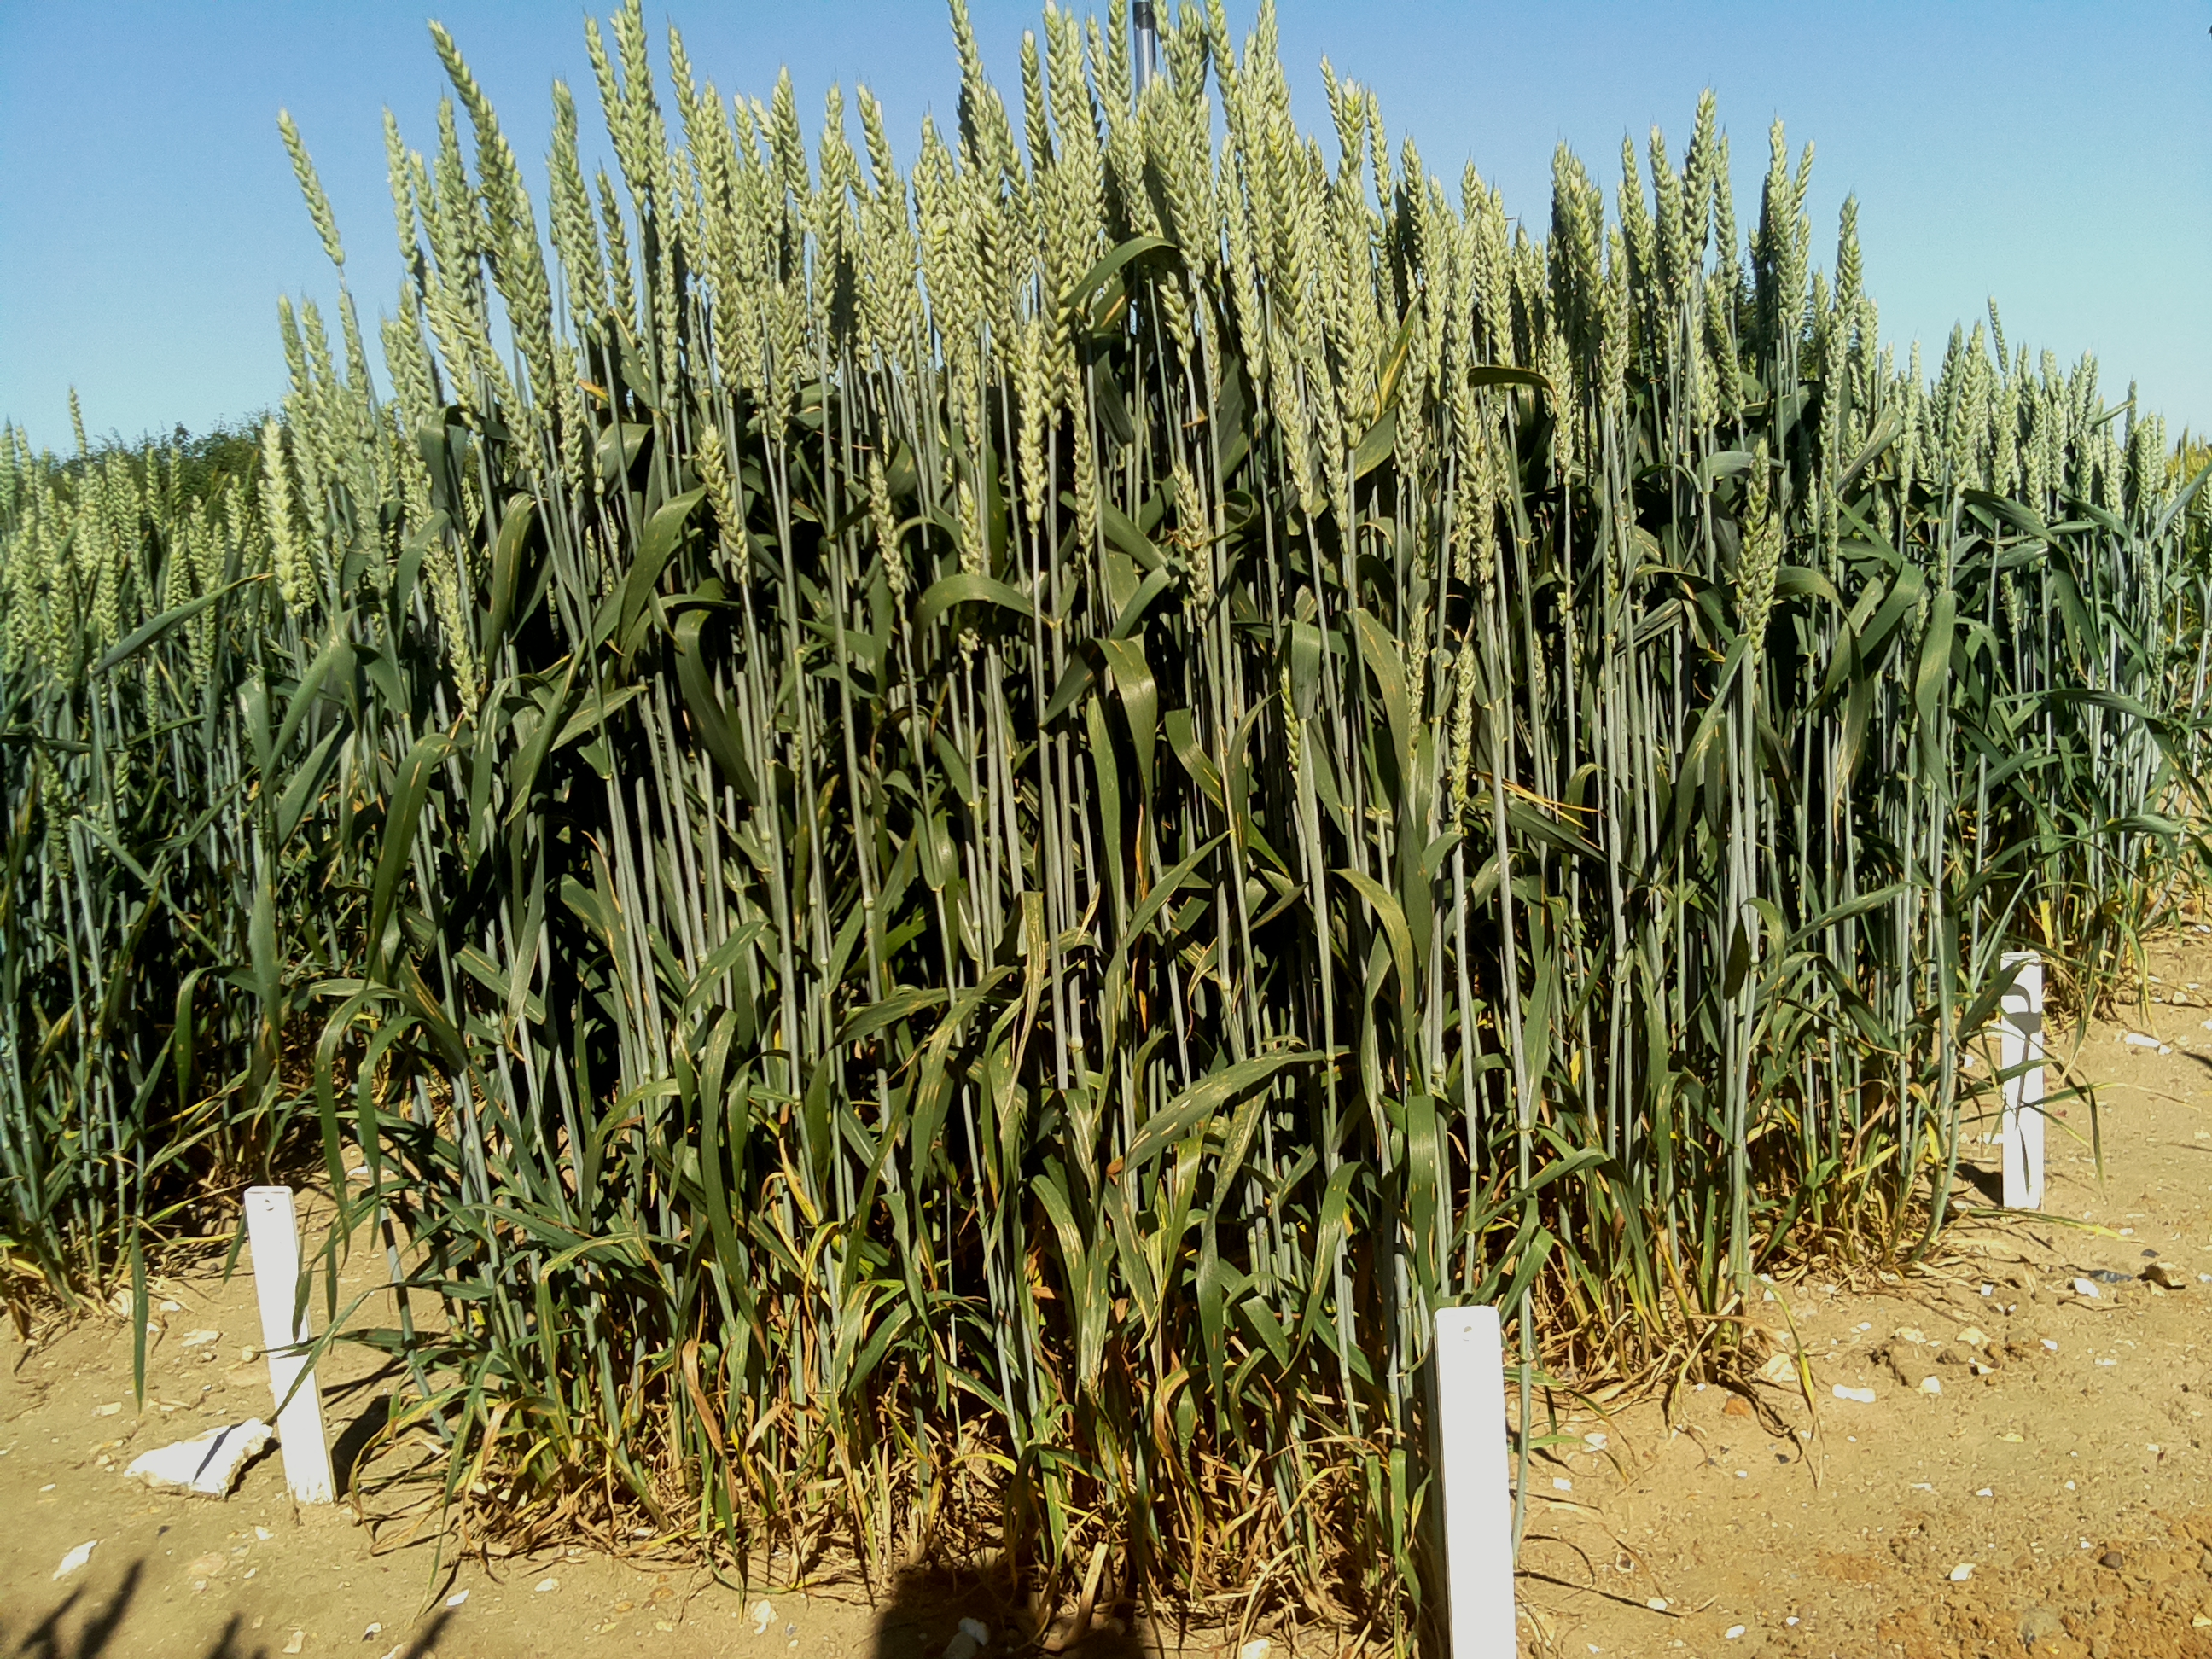
\includegraphics[width=\linewidth]{Images/005}
      \end{center}
    \end{minipage}
    &
    %\begin{minipage}[t]{5cm}
      xxx
    %\end{minipage}
    & 
    %\begin{minipage}{5cm}
      yyy
    %\end{minipage}
    & 
    %\begin{minipage}{5cm}
      zzz
    %\end{minipage}
    \\ \hline
    %%% NEW LINE %%%
    \begin{minipage}{.3\textwidth}
      \begin{center}
		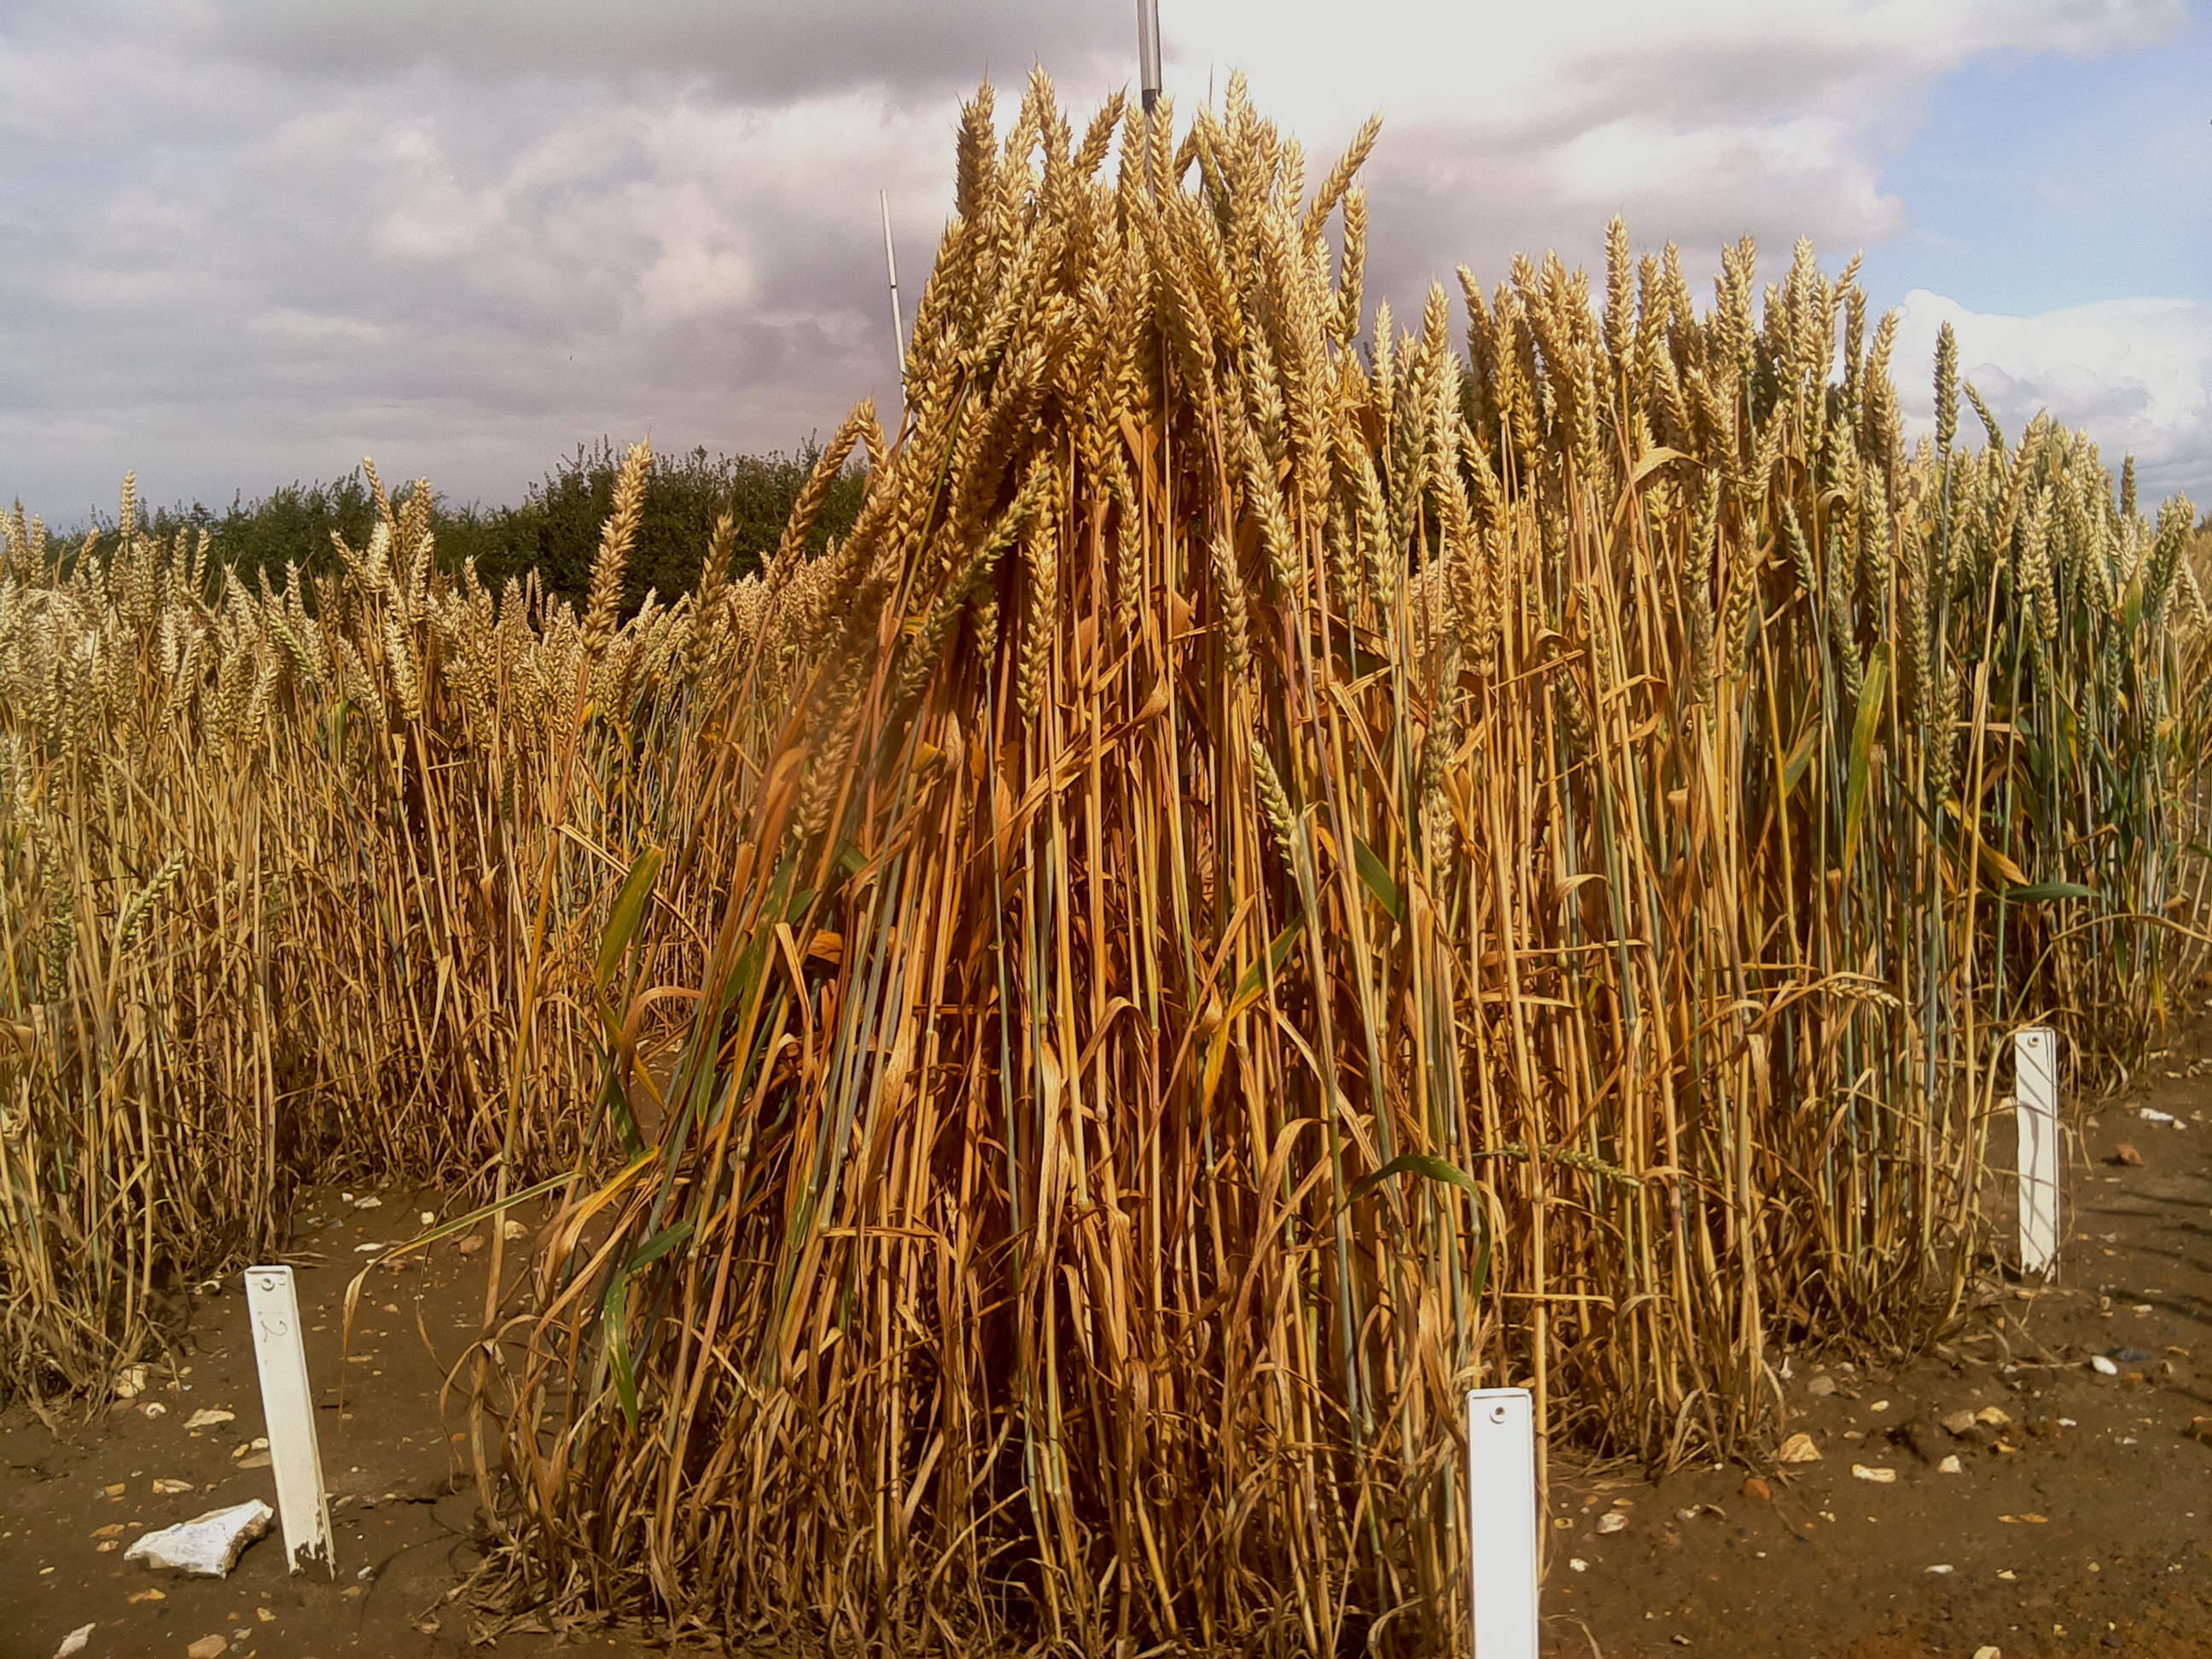
\includegraphics[width=\linewidth]{Images/006}
      \end{center}
    \end{minipage}
    &
    %\begin{minipage}[t]{5cm}
      xxx
    %\end{minipage}
    & 
    %\begin{minipage}{5cm}
      yyy
    %\end{minipage}
    & 
    %\begin{minipage}{5cm}
      zzz
    %\end{minipage}
    \\ \hline
  \end{tabular}
  \caption{Results of proposed system}\label{tbl:myLboro}
\end{table}

%%%%%%%%%%%%%%%%%%%%%%%%%%%%%%%%%%%%%%%%%%%%%%%%%%%%%%%%%%%%%
%%%% table pt 2 
%%%%%%%%%%%%%%%%%%%%%%%%%%%%%%%%%%%%%%%%%%%%%%%%%%%%%%%%%%%%%

\begin{table}[ht!]
  \centering
  \begin{tabular}{ | c | c | c | c |}
    \hline
    Image & Actual count & Predicted count & Time taken \\ \hline
    \begin{minipage}{.3\textwidth}
      \begin{center}
		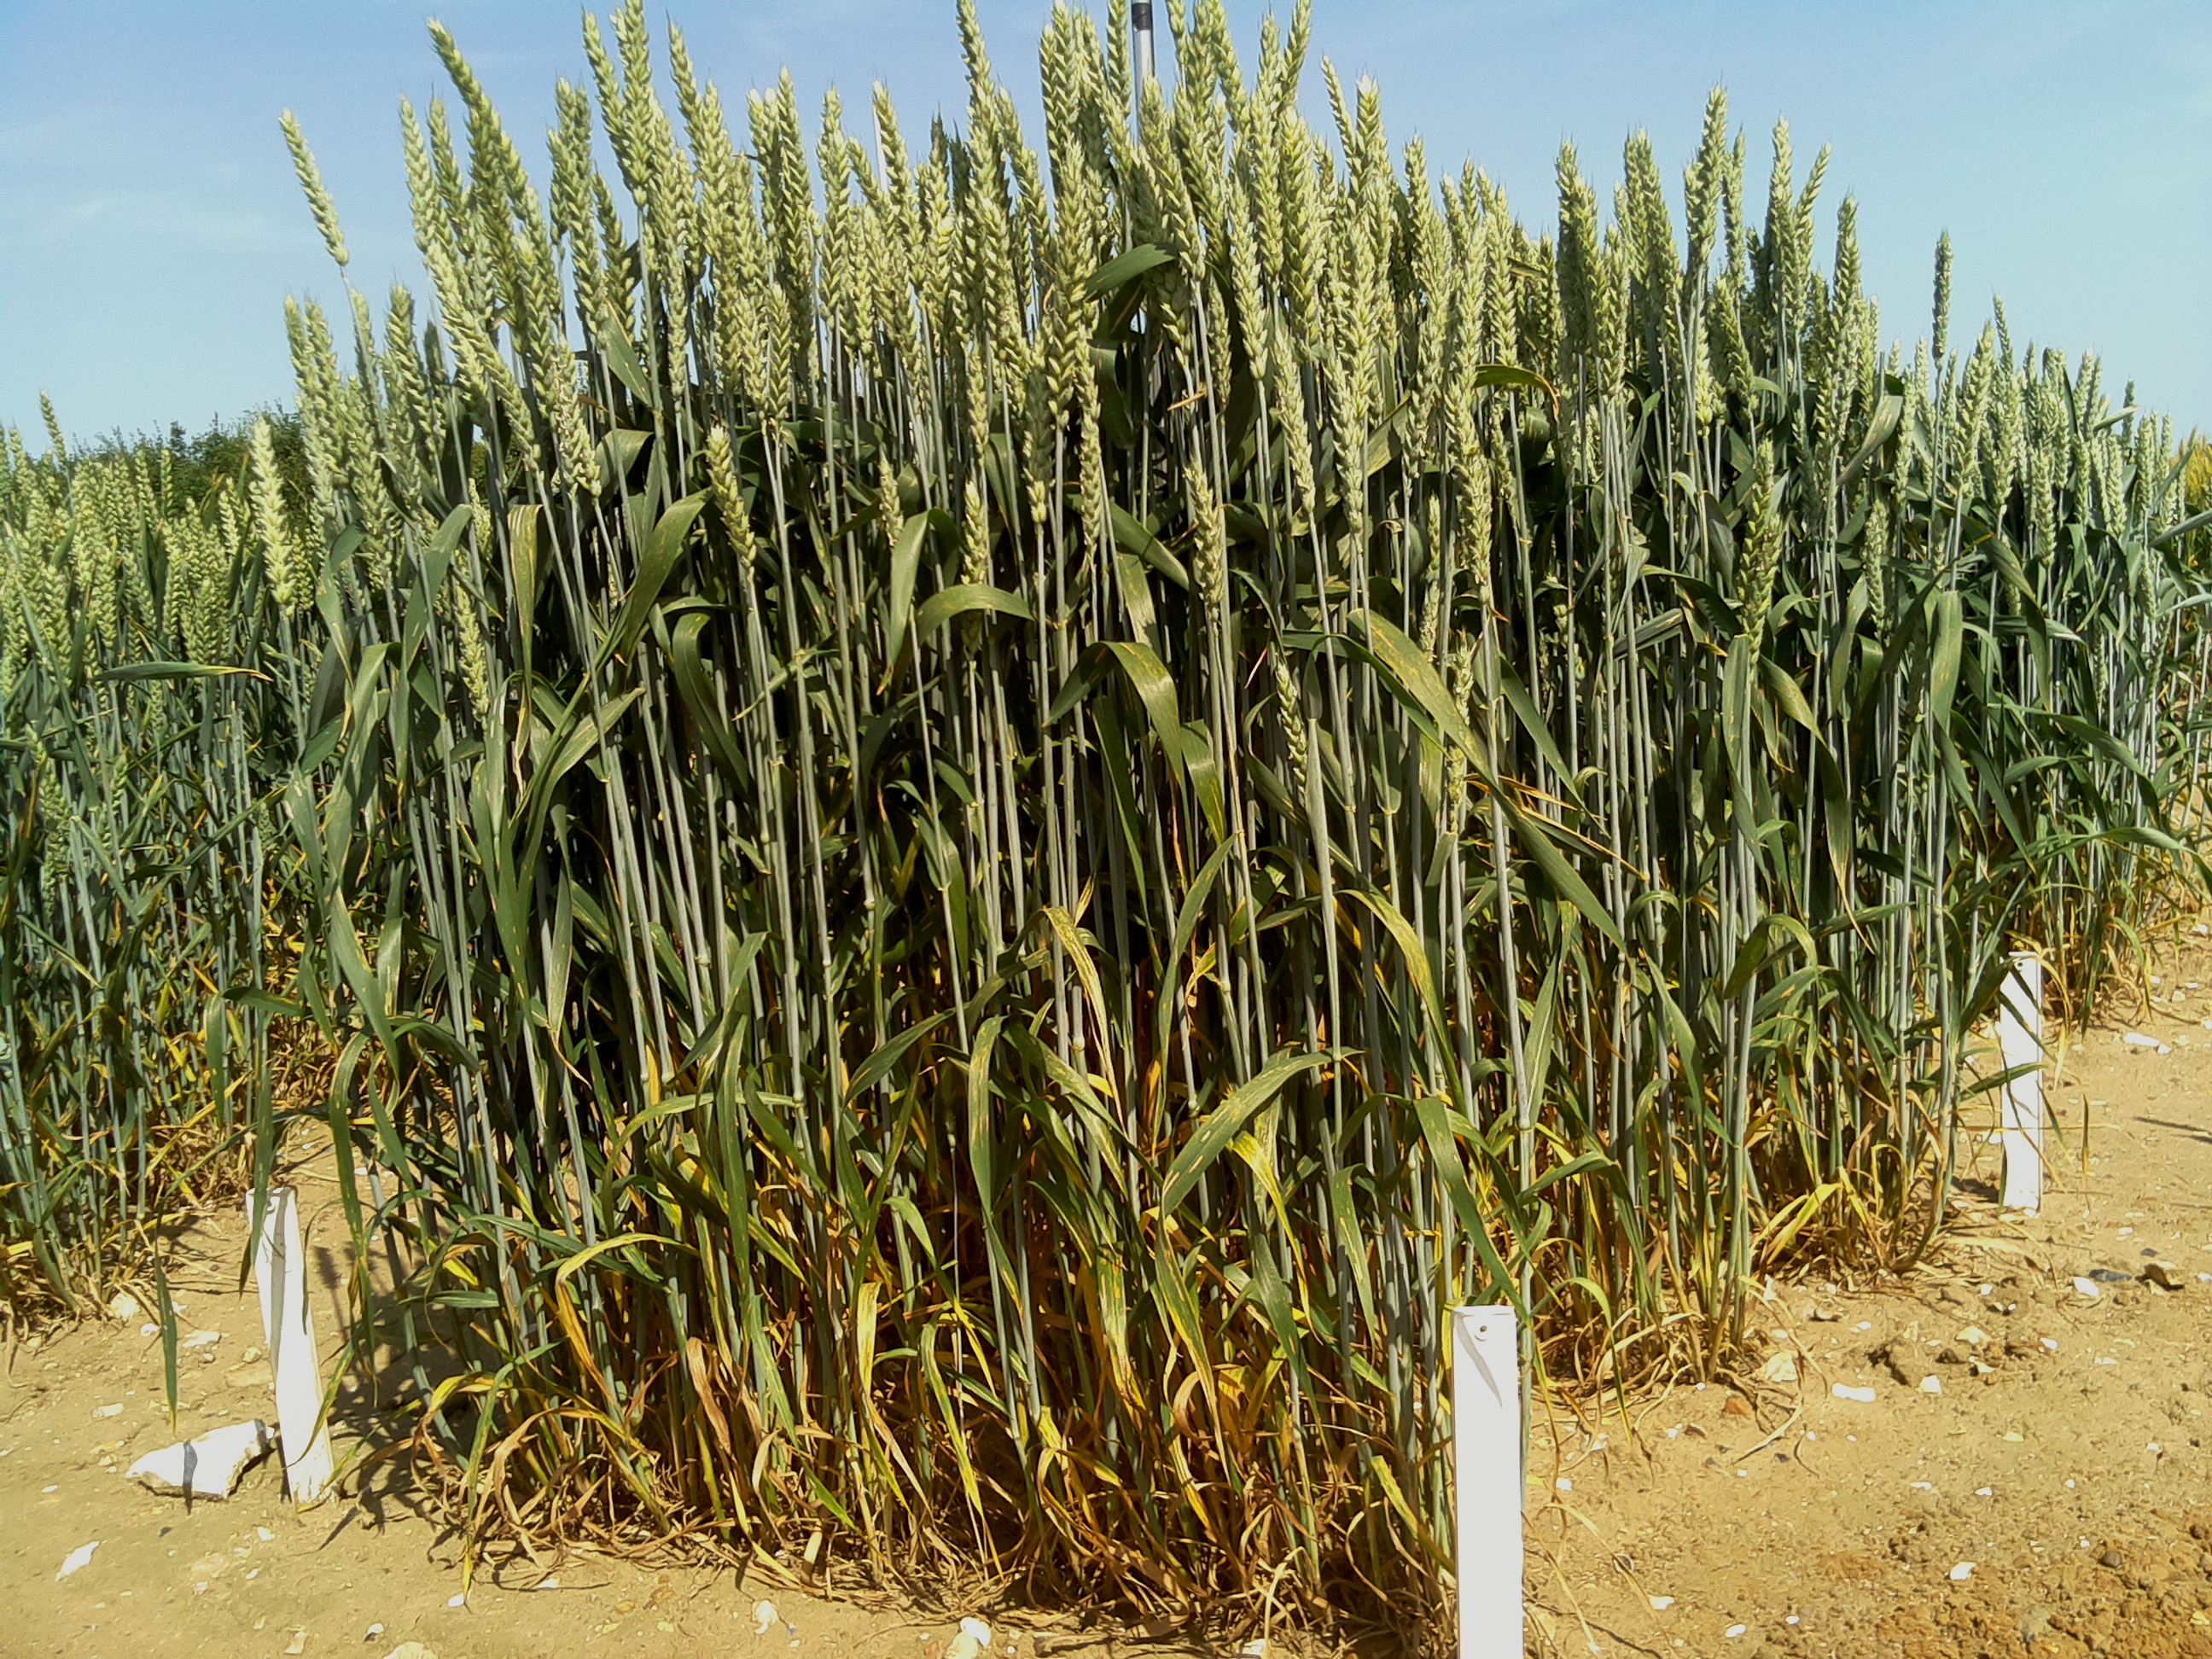
\includegraphics[width=\linewidth]{Images/008}
      \end{center}
    \end{minipage}
    &
    %\begin{minipage}[t]{5cm}
      xxx
    %\end{minipage}
    & 
    %\begin{minipage}{5cm}
      yyy
    %\end{minipage}
    & 
    %\begin{minipage}{5cm}
      zzz
    %\end{minipage}
    \\ \hline
    %%% NEW LINE %%%
    \begin{minipage}{.3\textwidth}
      \begin{center}
		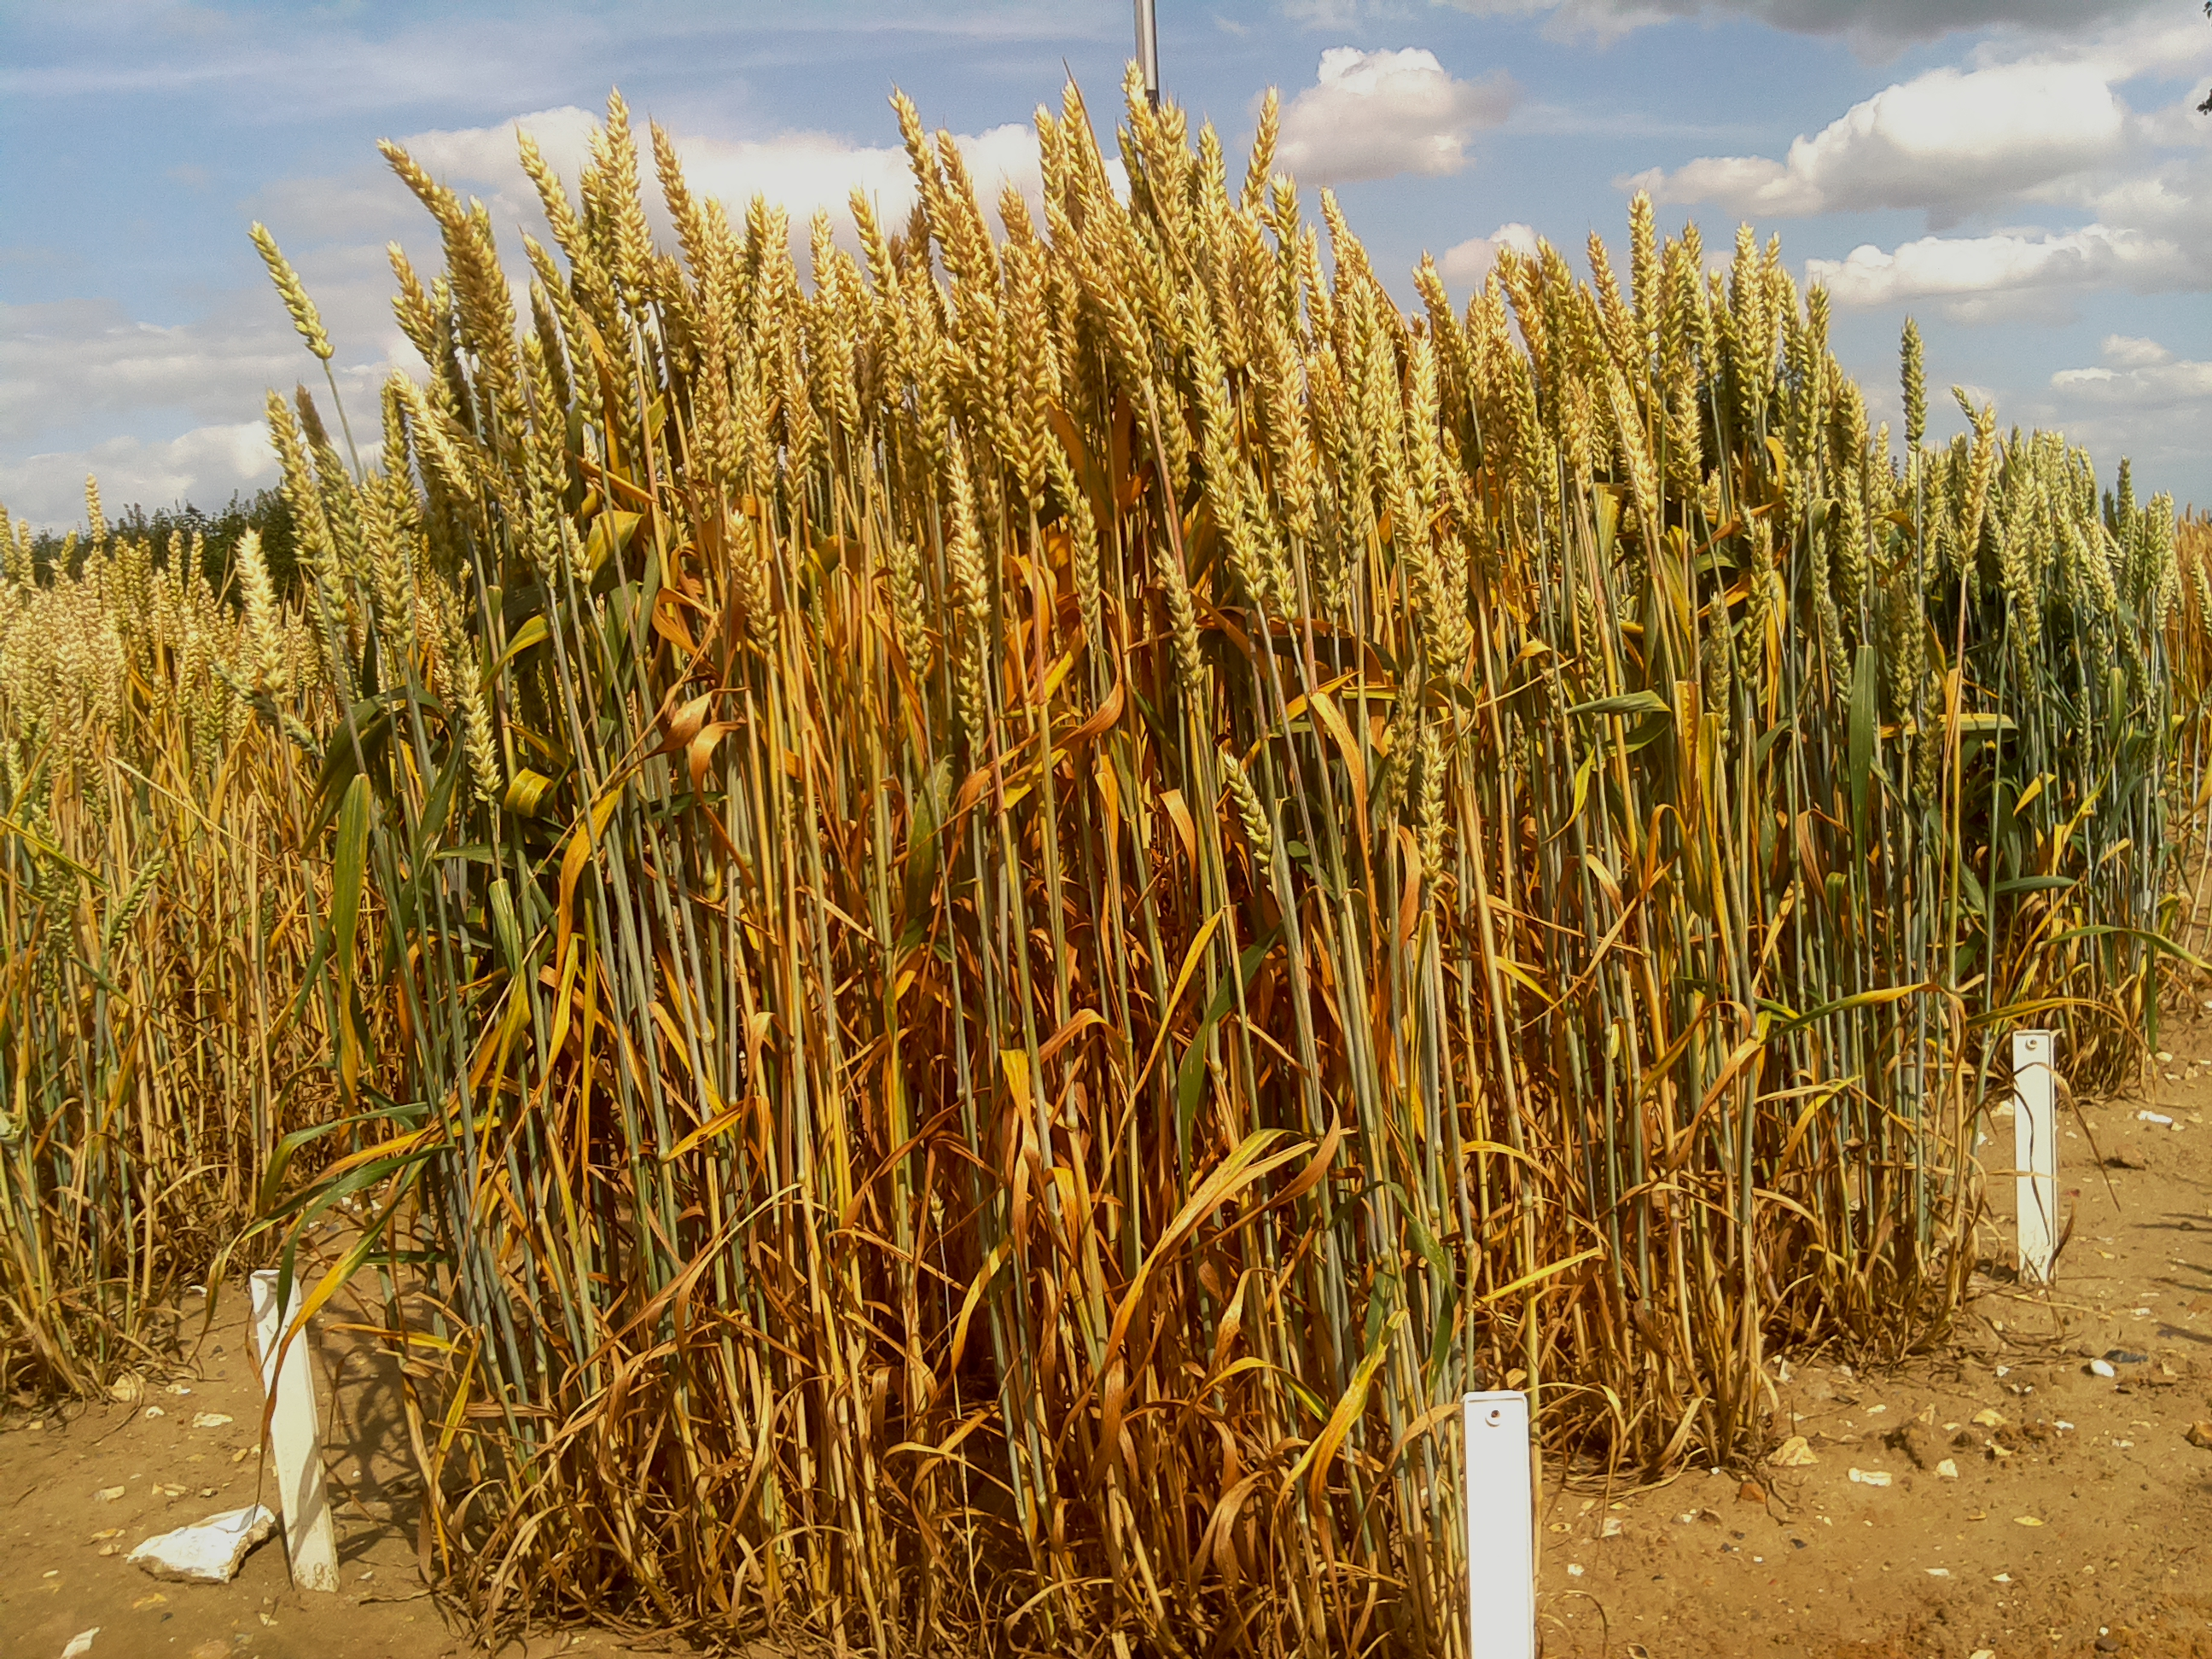
\includegraphics[width=\linewidth]{Images/009}
      \end{center}
    \end{minipage}
    &
    %\begin{minipage}[t]{5cm}
      xxx
    %\end{minipage}
    & 
    %\begin{minipage}{5cm}
      yyy
    %\end{minipage}
    & 
    %\begin{minipage}{5cm}
      zzz
    %\end{minipage}
    \\ \hline
    %%% NEW LINE %%%
    \begin{minipage}{.3\textwidth}
      \begin{center}
		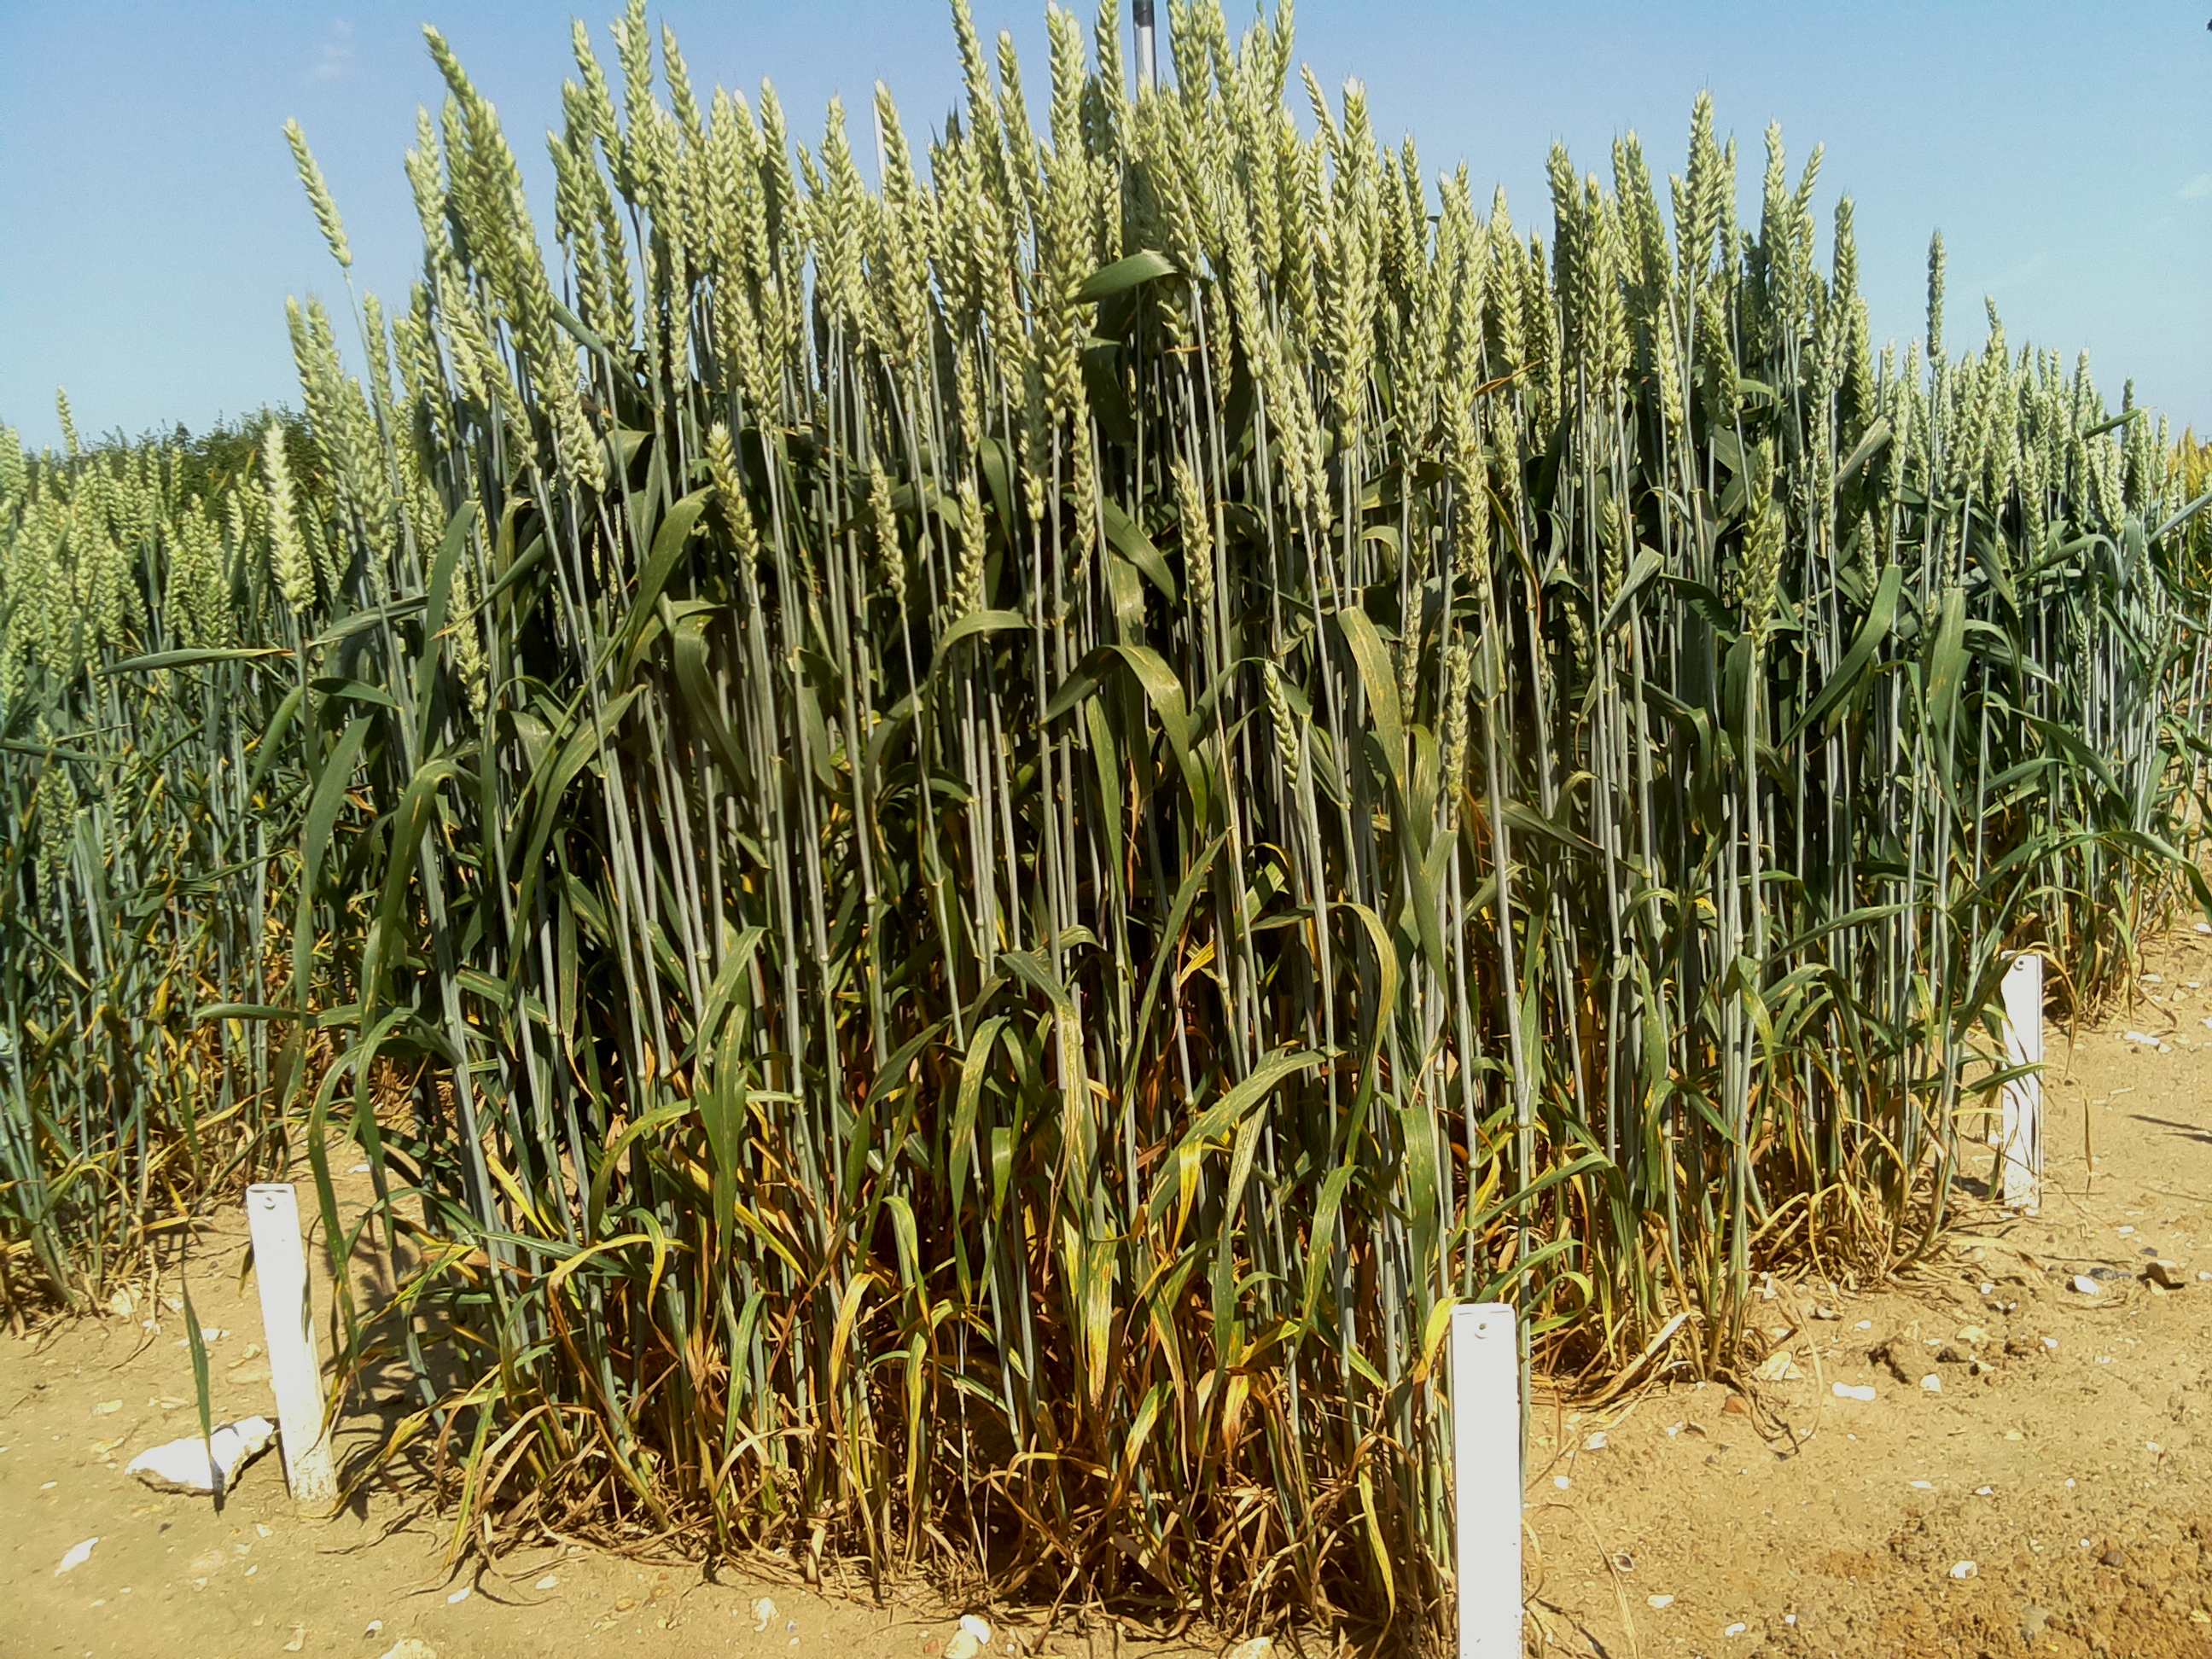
\includegraphics[width=\linewidth]{Images/010}
      \end{center}
    \end{minipage}
    &
    %\begin{minipage}[t]{5cm}
      xxx
    %\end{minipage}
    & 
    %\begin{minipage}{5cm}
      yyy
    %\end{minipage}
    & 
    %\begin{minipage}{5cm}
      zzz
    %\end{minipage}
    \\ \hline
    %%% NEW LINE %%%
    \begin{minipage}{.3\textwidth}
      \begin{center}
		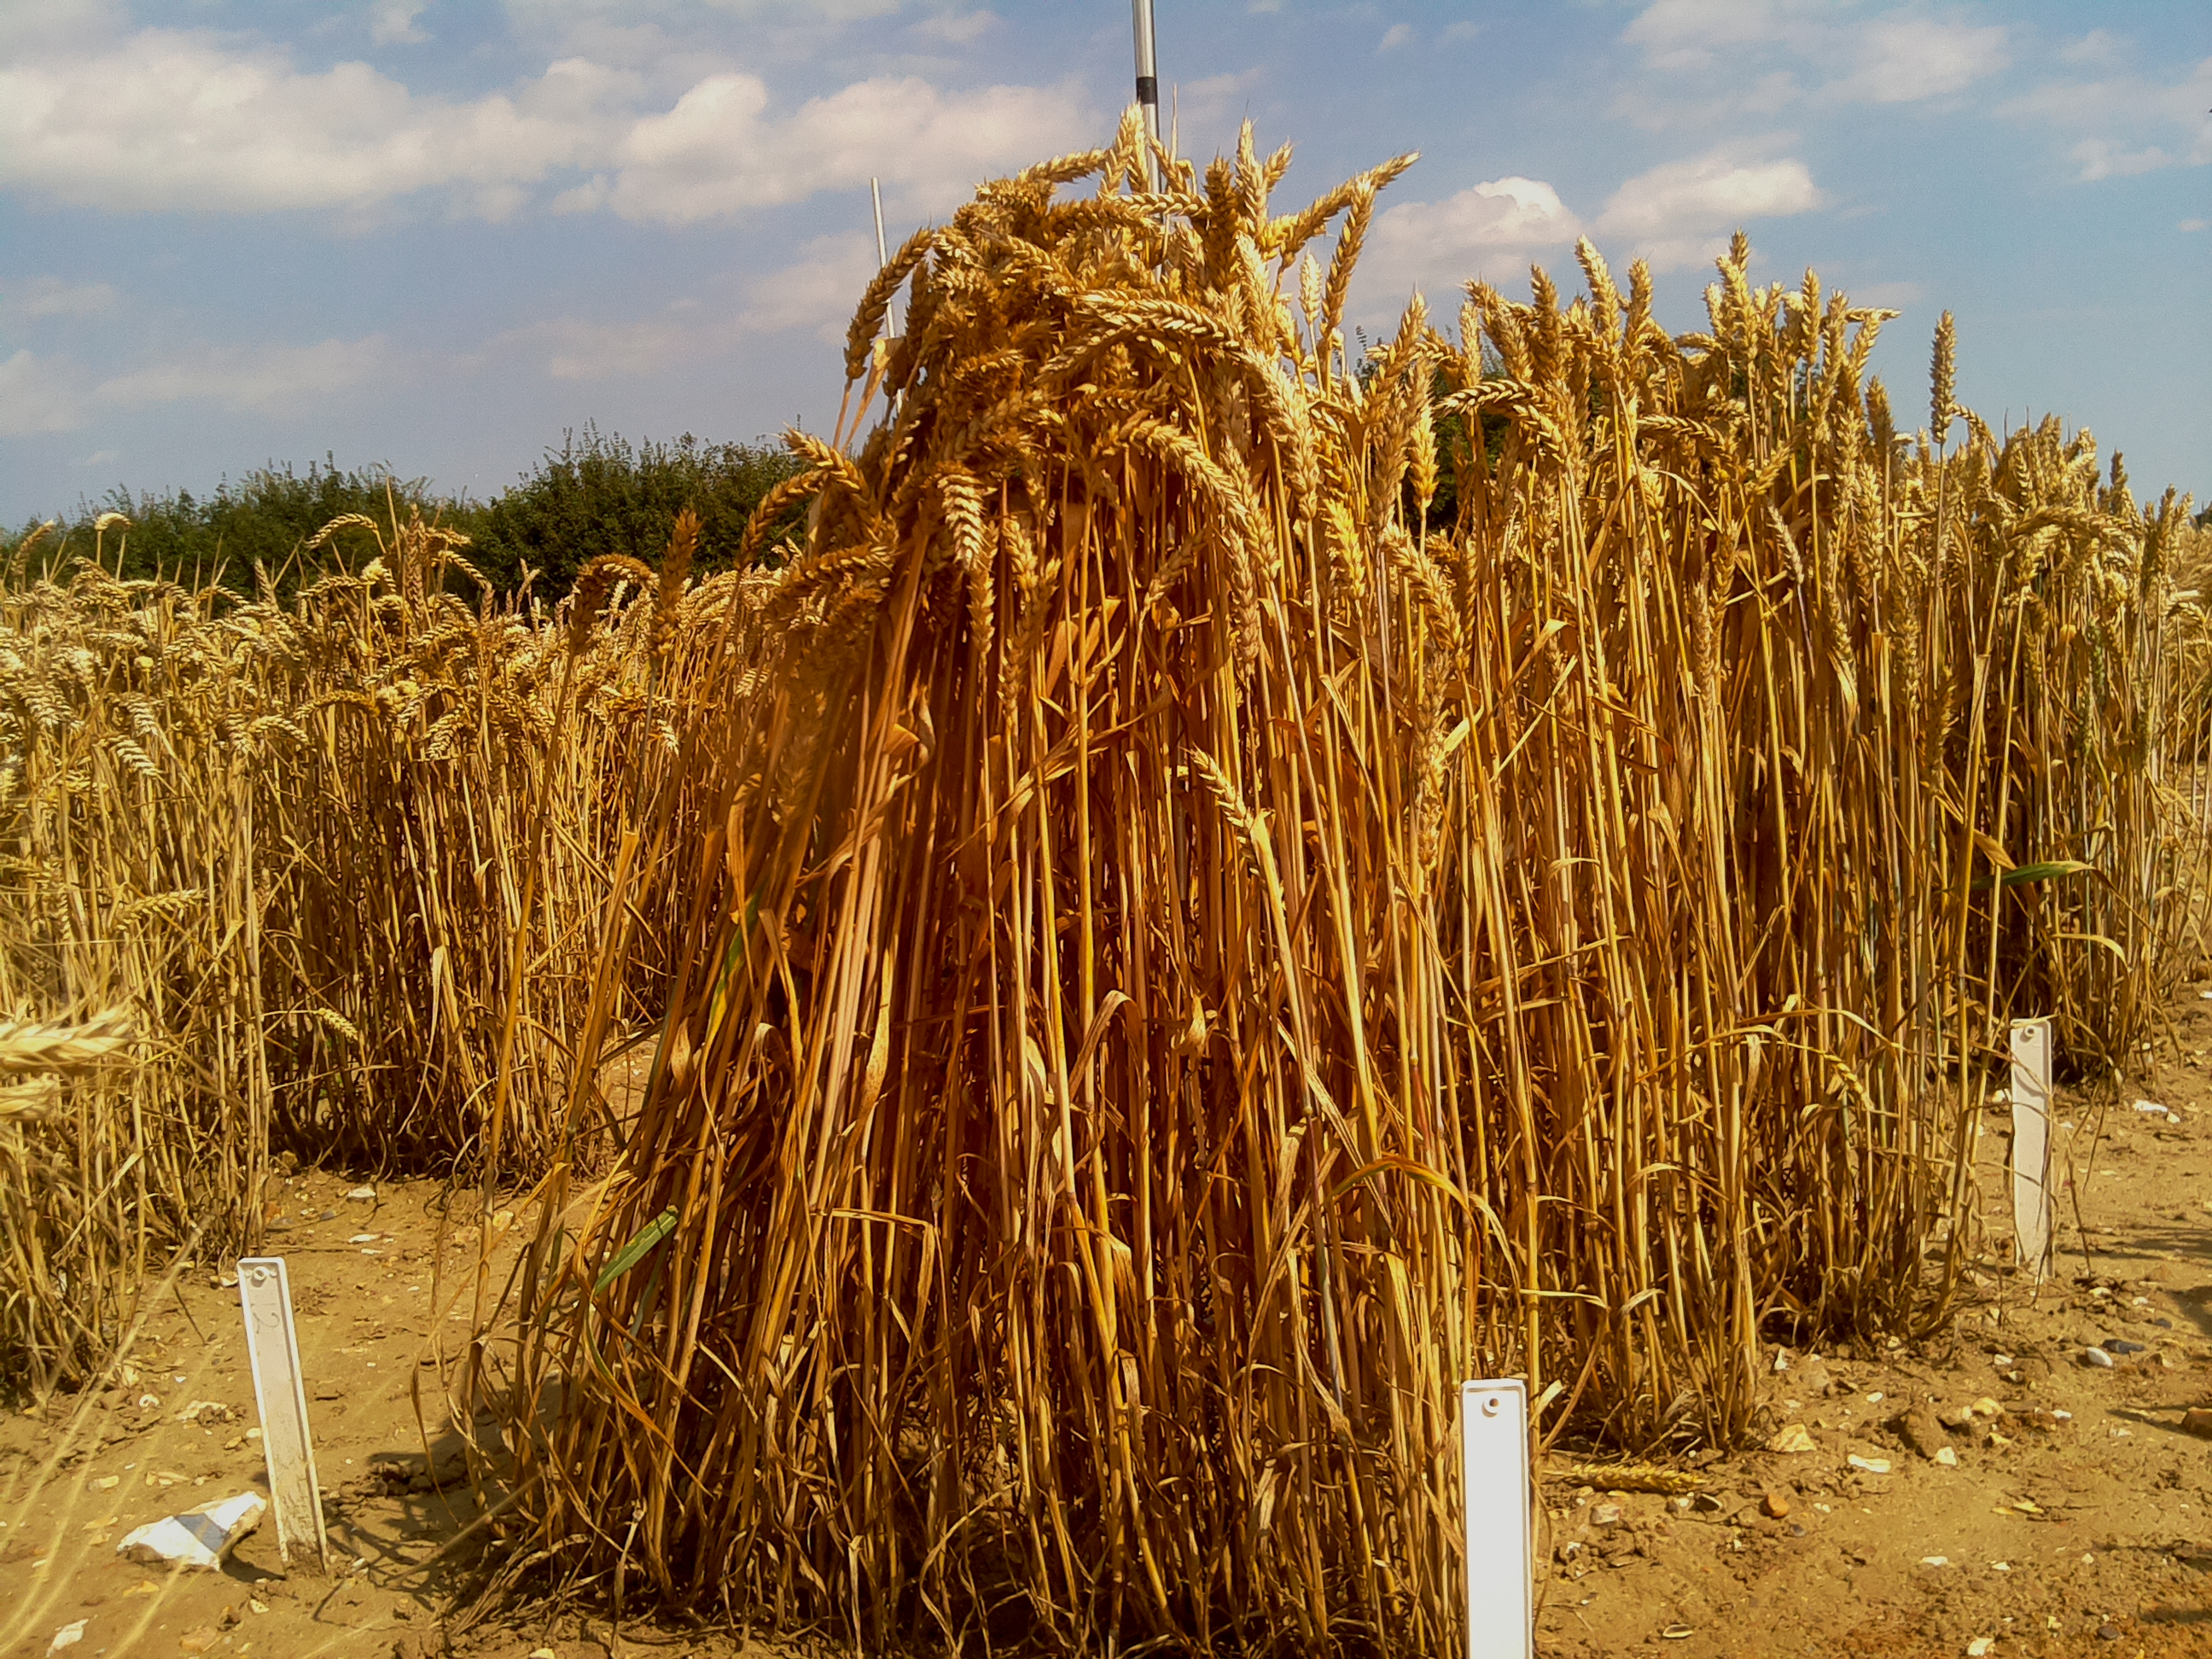
\includegraphics[width=\linewidth]{Images/011}
      \end{center}
    \end{minipage}
    &
    %\begin{minipage}[t]{5cm}
      xxx
    %\end{minipage}
    & 
    %\begin{minipage}{5cm}
      yyy
    %\end{minipage}
    & 
    %\begin{minipage}{5cm}
      zzz
    %\end{minipage}
    \\ \hline
    %%% NEW LINE %%%
    \begin{minipage}{.3\textwidth}
      \begin{center}
		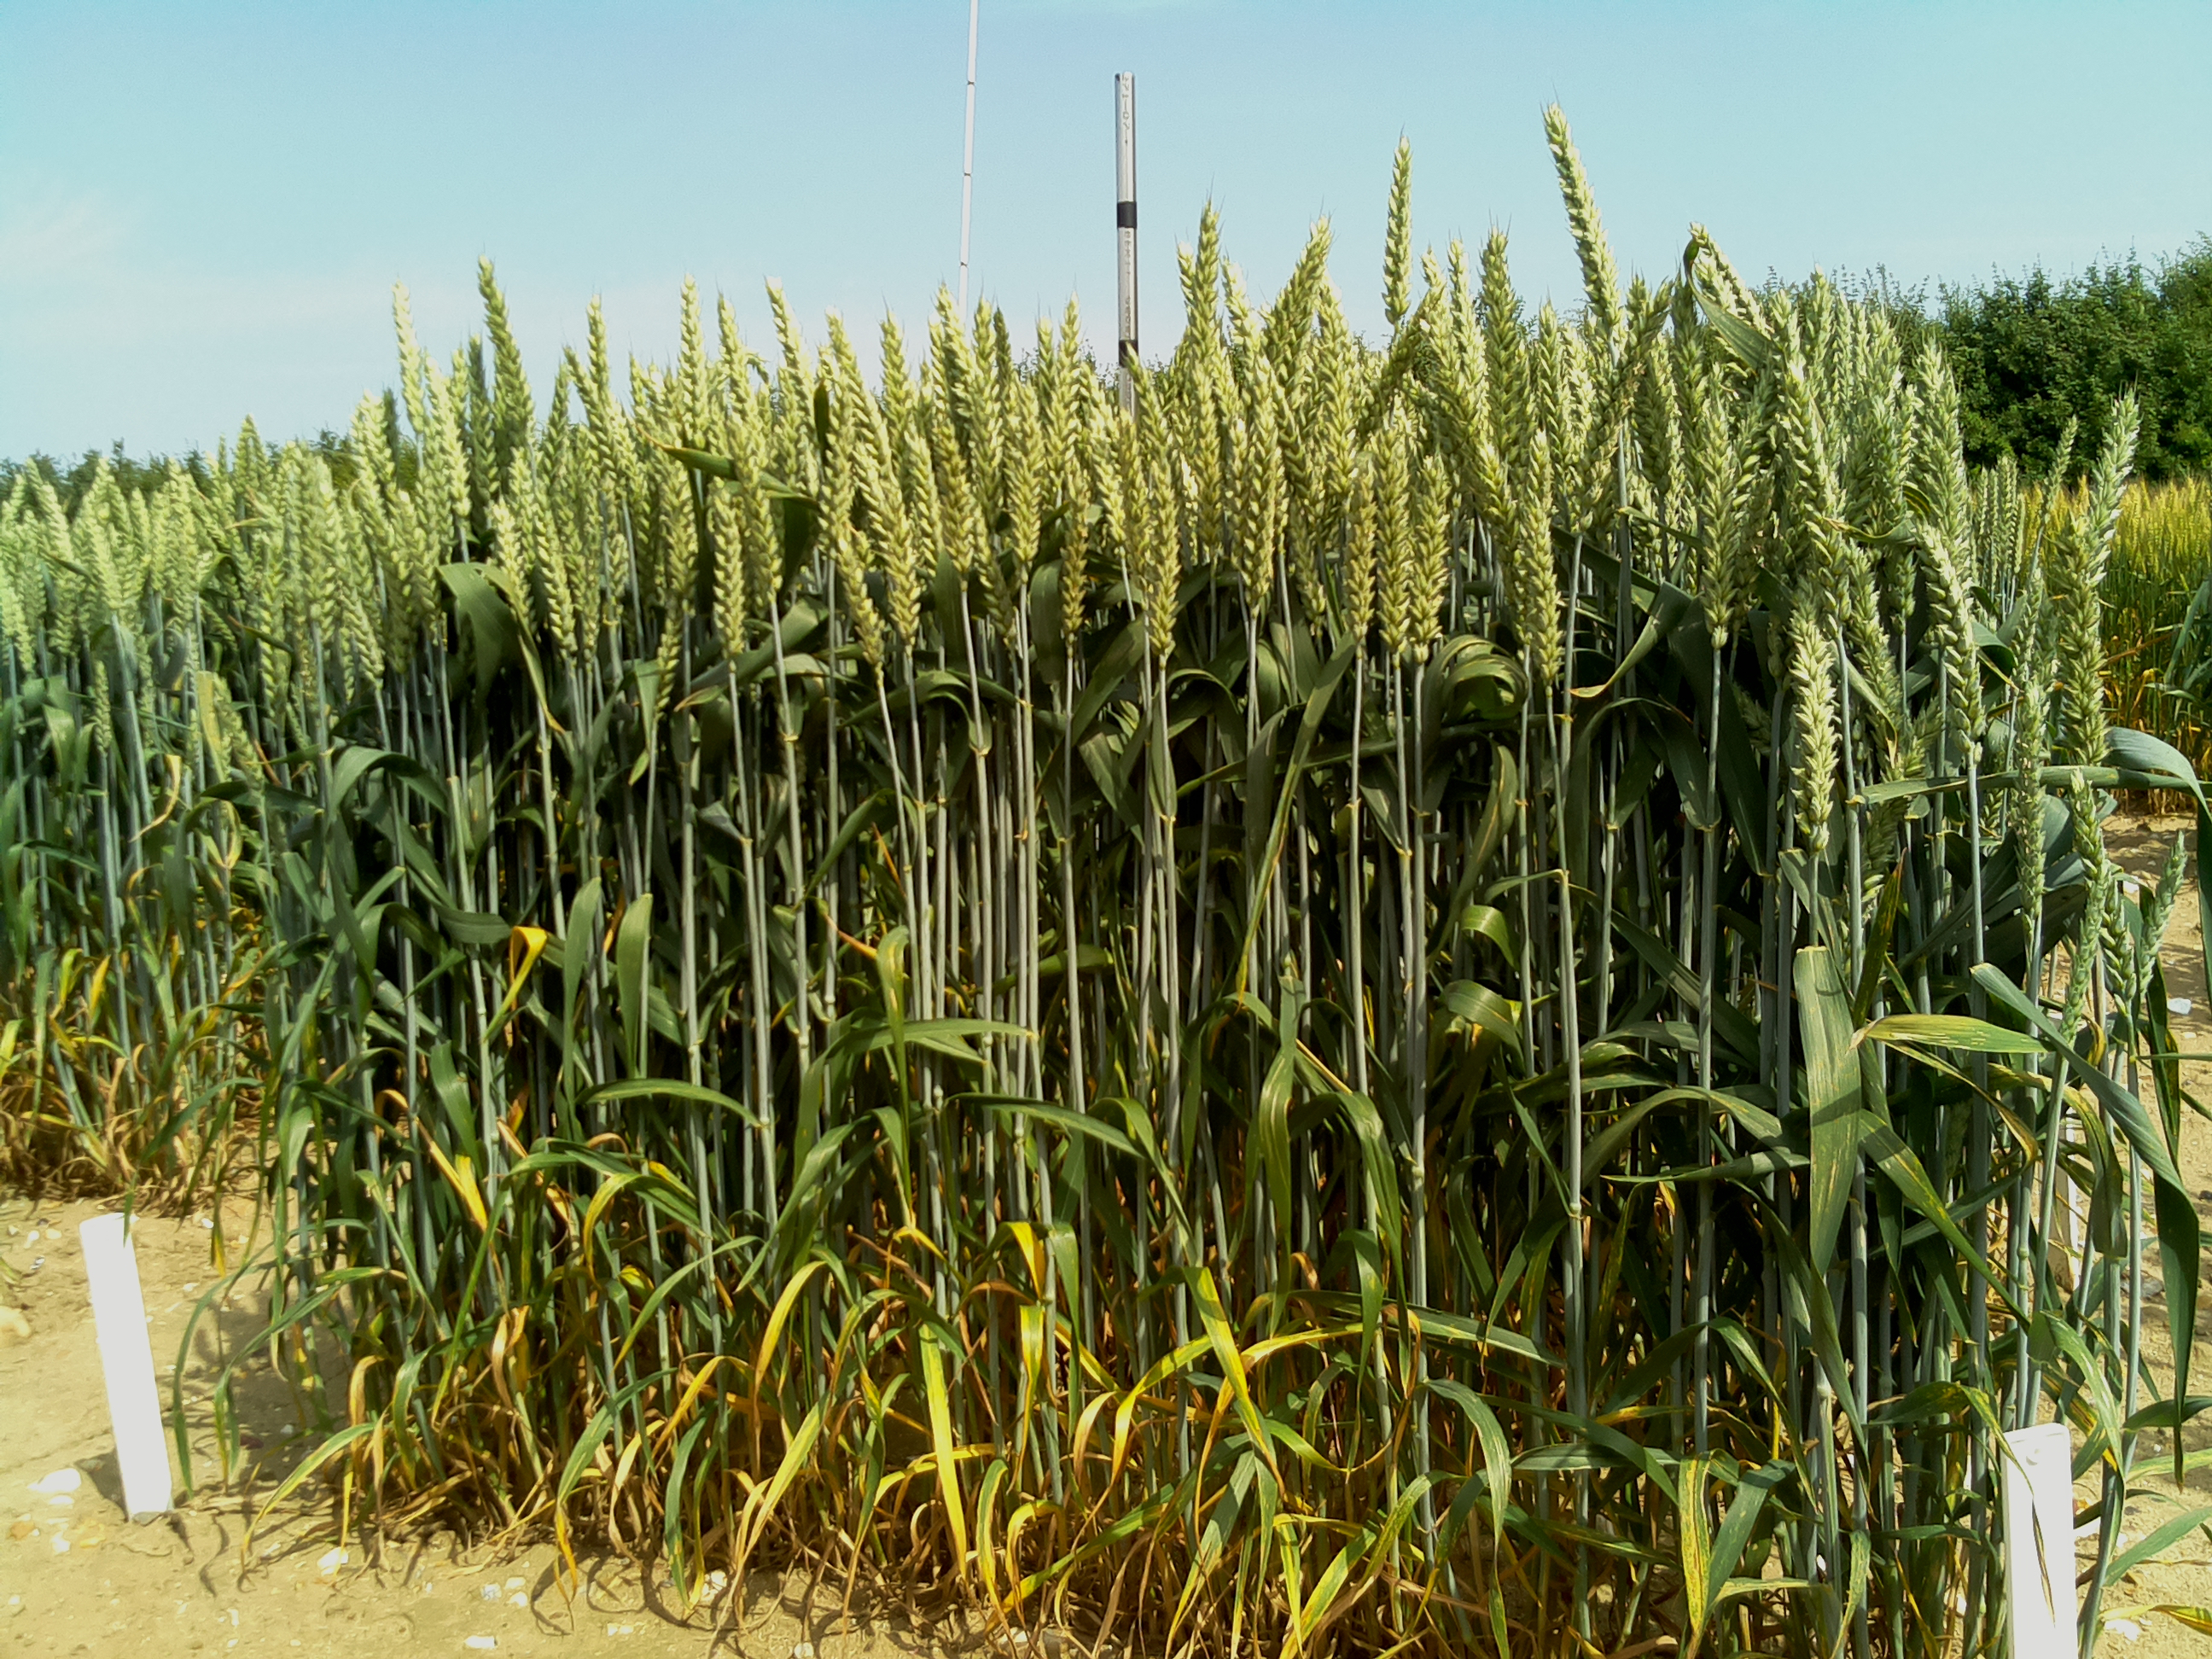
\includegraphics[width=\linewidth]{Images/012}
      \end{center}
    \end{minipage}
    &
    %\begin{minipage}[t]{5cm}
      xxx
    %\end{minipage}
    & 
    %\begin{minipage}{5cm}
      yyy
    %\end{minipage}
    & 
    %\begin{minipage}{5cm}
      zzz
    %\end{minipage}
    \\ \hline
    %%% NEW LINE %%%
  \end{tabular}
  \caption{Results of proposed system}\label{tbl:myLboro}
\end{table}
Having determined that the MLP could detect grains in images with an accuracy of $81.12\%$, it would be interesting to find out what this meant for the counting system itself. Tables 5.1 and 5.2 show the actual and predicted counts for the images provided as well as the time taken for the system to compute the counts. From these tables, it can be seen that the system seemed to perform better on some images than others. This was due to the fact that in the ROI extraction stage, the clusters to be extracted from the original image were hardcoded. This caused problems because the hardcoded clusters were not always the optimum (or sometimes even particularly good) clusters to select as regions of interest. A way around this problem would be to manually select the clusters denoting regions of interest to be extracted before before passing a query image to the system. A simple interactive program was built to this end. FIG\_ shows a screenshot of the ROI extraction interface. The program allows a user to upload an image and set the number of clusters that they wish to detect using the k-means clustering algorithm. The program then displays the image with the clusters overlayed over it and the user is able to select the clusters that they would like to extract. While this method might be slightly labour-intensive when a medium to large number of images need to have their grains counted, it yields much better performance. The trade-off here between labour-intensiveness and performance is something that would need to be considered in practice.
\begin{figure}[ht!]
\centering
\includegraphics[scale=0.7]{Images/gui}
\caption{Interactive program for manual ROI extraction}
\label{fig1}
\end{figure}

\bigskip

%%% ----------------------------------------------------------------------
\goodbreak

\section{Comparisons}
It was difficult to properly evaluate the counting-by-detection approach. While it showed poorer results by being off the actual count by more than the counting-by-detection method, it should be noted that it was trained on only 7 wheat images and tested on the remaining 6. Using only 7 images would definitely not have built a very good model. The counting-by-detection approach on the other hand had access to 5000 potential examples from each wheat image. Therefore, while the counting-by-detection approach out-performed the counting-by-regression approach, it is still too soon to write off the regression approach as being inferior. However, because we know the accuracy of regression approaches is limited as there is no universal function that can map images to grain counts for any and all images. If a system can correctly detect grains in images (of any kind) to a reasonable extent, such a system would outclass any built on regression approaches\\ \\
%
The system proposed relies on a machine learning classifier for grain detection. Our solution makes use of a neural network. We tried other classifiers to see how they all measured up. For image classification, neural networks and support vector machines perform best so the two were pit against each other in order to determine which was best for this problem. In particular, an MLP neural network and an SVM with the \textit{radial basis function} as the kernel function were used. While the SVM was hundreds of times faster than the neural network, it only yielded a prediction accuracy of $65.9\%$ while the neural network yielded an accuracy of $81.12\%$. Despite the fact that the SVM was able to count grains in a fraction of the time that the neural network did, the difference in prediction accuracy was too great to be disregarded in favour of speed. There are still more kinds of neural networks besides the MLP variation used in our solution and in the future, we intend to look into how they can be applied to the problem. Convolutional neural networks are one such example. 



\bigskip

%%% ----------------------------------------------------------------------




%% ------------------------------------------------------------------------
% -*-TeX-*- -*-Hard-*- Smart Wrapping
% ------------------------------------------------------------------------
\def\baselinestretch{1}

\chapter{Future Work}

\def\baselinestretch{1.66}






% ------------------------------------------------------------------------
% -*-TeX-*- -*-Hard-*- Smart Wrapping
% ------------------------------------------------------------------------
\def\baselinestretch{1}

\chapter{Conclusion}

\def\baselinestretch{1.66}







% ------------------------------------------------------------------------
\setlinespacing{1.44}
%\bibliographystyle{amsplain}
\bibliographystyle{apalike}
\bibliography{XBib}

%#### Include any appendix below #####
\appendix
%% ------------------------------------------------------------------------
% -*-TeX-*- -*-Hard-*- Smart Wrapping
% ------------------------------------------------------------------------
\def\baselinestretch{1}

\chapter{On Invariant Subspaces of Essentially Self--Adjoint Operators}

\def\baselinestretch{1.66}

%%% ----------------------------------------------------------------------

An application of the main result of the previous chapter to
the algebra generated by an essentially self--adjoint operator
$A$ yields the existence of nonzero vectors $x,y\in\h$ such
that $\tau(p)=\seq{p(A)x,y}$ is a positive functional on the
space of all polynomials on the essential spectrum of $A$. This
result immediately implies the existence of real invariant
subspaces for essentially self--adjoint operators acting on a
complex Hilbert space. Elementary convex analysis techniques,
applied to the space of certain vector states, yield the
existence of invariant subspaces for essentially self--adjoint
operators acting on an infinite--dimensional real Hilbert
space.

%%% ----------------------------------------------------------------------
\goodbreak
\section{Introduction}

The existence of invariant subspaces for compact perturbations
of self--adjoint operators appears to be one of the most
difficult questions in the theory of invariant
subspaces~\cite{Lom92}. The positive results about the
existence of the invariant subspaces for the Schatten--class
perturbations of self--adjoint operators, acting on a complex
Hilbert space, date back to the late 1950's. For the facts
concerning such operators see Chapter~6 in~\cite{RR73}, where a
brief history of the problem, together with the references to
the related topics is given. The proofs of those results are
based on the concept of the separation of spectra. However,
Ljubi\v{c} and Macaev~\cite{LM65} showed that there is no
general spectral theory by constructing an example of an
operator $A$ such that $\sigma(A|\cal{M})=[0,1]$ whenever
$\cal{M}$ is a nonzero invariant subspace for $A$. This
suggests that different techniques might be needed to establish
the existence of invariant subspaces for essentially
self--adjoint operators.

\smallskip

The fact that the right--hand side of the
inequality~(\ref{e:ESSCON}) depends only on the essential norm
of the real part of the operator $A$, suggests that
Proposition~\ref{p:ESS} might have applications to the
invariant subspace problem for compact perturbations of
self--adjoint operators. In this chapter we apply
Proposition~\ref{p:ESS} in order to construct positive
functionals $\tau(p)=\seq{p(A)x,y}$ on the space of all
polynomials restricted to the essential spectrum of $A$.
Finally, in the case when the underlying Hilbert space is real,
the existence of invariant subspaces for $A$ is established
after solving an extreme problem concerning certain convex
subspaces of vector states.

\begin{defn}
Suppose $\h$ is a real or complex Hilbert space. An operator
$A\in\BH$ is called \emph{essentially self--adjoint}, if
$\pi(A)$ is a self--adjoint element in the Calkin algebra
$\BH/\KH$, where $\pi\colon\BH\To\BH/\KH$ is the quotient
mapping.
\end{defn}

\begin{rem}
Clearly, by definition of the Calkin algebra, $A$ is
essentially self--adjoint if and only if $A=S+K$, where
$S\in\BH$ is self--adjoint and $K$ is a compact operator.
Hence, saying that $A$ is essentially self--adjoint, is the
same as saying that $A$ is a compact perturbation of a
self--adjoint operator. Note, however, that this is
{\em{}false} if we replace self--adjoint operators by normal
ones.
\end{rem}

%%% ----------------------------------------------------------------------
\goodbreak
\section{On Real Invariant Subspaces}

Recently V.I.~Lomonosov~\cite{Lom92} proved that every
essentially self--adjoint operator acting on a complex Hilbert
space has a nontrivial closed \emph{real} invariant subspace.
We give an alternative proof, based on Proposition~\ref{p:ESS},
and thus introduce the idea that will be later generalized in
order to yield the existence of proper invariant subspaces for
essentially self--adjoint operators acting on a real Hilbert
space.

Recall that a \emph{real subspace} of a complex Hilbert space
$\h$ is a subset that is closed under addition and
multiplication by the \emph{real} scalars. A real subspace
$\cal{M}\subset\h$ is invariant for an operator $A\in\BH$ if
and only if $\cal{M}$ is invariant under all operators in the
\emph{real} algebra generated by $A$, i.e. the algebra of all
real polynomials in $A$.

\begin{prop}\label{p:RIS}
Suppose $\h$ is an infinite--dimensional complex Hilbert space
and let $\A$ be a convex set of commuting essentially
self--adjoint operators. Then the set of non--cyclic vectors
for $\A$ is dense in $\h$.
\end{prop}

\begin{proof}
Suppose not; then there exists a unit vector $f_0$ and a
positive number $r\in(0,1)$ such that all vectors in the set
\[  \s=\set{f\in\h\,\,|\,\,\,\norm{f_0-f}\leq\tfrac{r}{\sqrt{1-r^2}}}, \]
are cyclic for $\A$. In particular, for every vector $g\in\h$
and $\norm{g}\leq1$, there exists an operator $A\in\A$ such
that
\[ \RE\seq{A\left(f_0+\tfrac{r}{\sqrt{1-r^2}}g\right),
          -i\left(f_0-\tfrac{\sqrt{1-r^2}}{r}g\right)} > 0, \]
or equivalently,
\[ \RE\seq{ i A\left(f_0+\tfrac{r}{\sqrt{1-r^2}}g\right),
                     f_0-\tfrac{\sqrt{1-r^2}}{r}g} > 0. \]
Since $A$ is an essentially self--adjoint operator, it follows
that
\[ \essnorm{\IM{A}}=\essnorm{\RE(i{A})}=0, \]
and consequently the convex set
$i\A=\set{i{A}\,\,|\,\,\,A\in\A}$, satisfies the hypothesis of
Proposition~\ref{p:ESS}. Therefore, there exists an element
$A_0\in\A$ ($A_0\neq{z}I$), with an eigenvector $f_1\in\s$.
Since the operators in $\A$ commute, $f_1$ cannot be a cyclic
vector for $\A$, contradicting the assumption that all vectors
in $\s$ are cyclic for $\A$.
\end{proof}

\begin{cor}[V.I.\,Lomonosov, 1992]
Every essentially self--adjoint operator on an
infinite--dimensional complex Hilbert space has a nontrivial
closed real invariant subspace.
\end{cor}

\begin{proof}
The commutative algebra $\A_{\Real}$ of all real polynomials in
$A$ consists of essentially self--adjoint operators whenever
$A$ is essentially self--adjoint. By Proposition~\ref{p:RIS}
the set of non--cyclic vectors for $\A_{\Real}$ is dense in
$\h$. Since for every nonzero vector $f\in\h$ the closure of
the orbit $\A_{\Real}f=\set{T{f}\,\,|\,\,\,T\in\A_{\Real}}$ is
a real invariant subspace for $A$, it follows that $A$ has a
nontrivial closed real invariant subspace.
\end{proof}

\begin{rem}
If $A$ is a self--adjoint operator acting on a complex Hilbert
space $\h$, then for every vector $f\in\h$ and every real
polynomial $p$ we have:
\begin{equation} \label{e:I0}
  \IM\seq{p(A){f},f}=0.
\end{equation}
The condition (\ref{e:I0}) in fact characterizes self--adjoint
operators on a complex Hilbert space~\cite[p.~103]{KR83}.
Roughly speaking, Proposition~\ref{p:RIS} and its corollary
establish a similar fact for essentially self--adjoint
operators acting on a complex Hilbert space.
\end{rem}

%%% ----------------------------------------------------------------------
\goodbreak
\section{The Space of Vector States}

In the previous section we applied our machinery only to the
imaginary part of an essentially self--adjoint operator $A$. An
application to the real part yields the existence of ``vector
states'' on the space of all polynomials restricted to the
essential spectrum of $A$. Before proceeding, we make the
following conventions that hold through the rest of this
chapter:

\bigskip

As usual, let $\h$ be an infinite--dimensional real or complex
Hilbert space. The underlying field of real or complex numbers
(respectively) is denoted by $\Field$. Suppose $A\in\BH$ is a
fixed essentially self--adjoint operator without non--trivial
closed invariant subspaces and let $E$ denote its essential
spectrum. Furthermore, we may assume that $\essnorm{A}\leq1$,
and consequently, $E\subset[-1,1]$. Let $\A\subset\BH$ be an
algebra generated by $A$, i.e. $\A$ is the algebra of all
polynomials $p(A)$ with the coefficients in the underlying
field $\Field$.

\medskip

\noindent The algebra of all polynomials with the coefficients
in $\Field$, equipped with the norm
\[ \norm{p}_\infty=\max_{t\in{E}} \abs{p(t)}, \]
is denoted by $\Poly$.

\smallskip

\begin{defn}
Let $\EssD\subset\h$ be the set of all nonzero vectors $x\in\h$
for which there exists a nonzero vector $y\in\h$ satisfying the
following inequality for every polynomial $p\in\Poly$
\begin{equation} \label{e:PF1}
  \RE\seq{p(A)x,y} \leq \norm{\RE p}_\infty\seq{x,y}.
\end{equation}
\end{defn}

\medskip

\goodbreak

\begin{lem}\label{l:PF1}
The set $\EssD$ is dense in $\h$.
\end{lem}

\begin{proof}
Since the operator $A$ has no invariant subspaces the condition
of Proposition~\ref{p:ESS} is never satisfied for the algebra
$\A$. More precisely, for every unit vector $f_0\in\h$ and any
positive number $r\in(0,1)$ there exists a vector $g\perp{}f_0$
such that for every polynomial $p\in\Poly$
\[ \RE\seq{p(A)\left(f_0+\tfrac{r}{\sqrt{1-r^2}}g\right),
                  f_0-\tfrac{\sqrt{1-r^2}}{r}g} \leq
   \essnorm{\RE{}p(A)}(1 - \norm{g}^2). \]
Clearly, for every polynomial $p\in\Poly$ we have
\[ \essnorm{\RE p(A)} = \essnorm{(\RE p)(A)} = \norm{\RE p}_\infty. \]
The vectors
\[ x=f_0+\tfrac{r}{\sqrt{1-r^2}}g
   \quad \text{ and } \quad
   y=f_0-\tfrac{\sqrt{1-r^2}}{r}g \]
satisfy the inequality (\ref{e:PF1}). Letting $r\to0$, and
replacing the vector $x$ by $\lambda{x}$, where $\lambda>0$,
implies the required density of $\EssD$.
\end{proof}

\begin{lem} \label{l:PF2}
For fixed vectors $x,y\in\h$ define a linear functional
$\tau\colon\Poly\To\Field$
\[ \tau(p) = \seq{p(A)x,y}. \]
Then $\tau$ is a bounded positive functional on the space
$\Poly$ if and only if the following inequality is satisfied
for every polynomial $p\in\Poly$:
\[ \RE\seq{p(A)x,y} \leq \norm{\RE p}_\infty\seq{x,y}. \]
\end{lem}

\begin{proof}
Suppose that $\tau$ is a positive functional on $\Poly$. Then
$\RE \seq{p(A)x,y} = \seq{(\RE p)(A)x,y}$. Since $\norm{\RE
p}_\infty - \RE p$ is a positive polynomial on $E$, we have
\[ \tau(\norm{\RE p}_\infty - \RE p) =
   \seq{(\norm{\RE p}_\infty - \RE p)(A)x, y} \geq 0, \]
or equivalently,
\[ \RE\seq{p(A)x,y} \leq \norm{\RE p}_\infty\seq{x,y}. \]

Conversely, suppose $\tau$ is not a bounded positive functional
on $\Poly$. Then either there exists a real polynomial $p$ such
that $\IM\seq{p(A)x,y}\neq0$, or $\seq{p(A)x,y}<0$ for some
positive polynomial $p\in\Poly$. After replacing $p$ by $\pm i
p$ it is easy to see that $\IM\seq{p(A)x,y}\neq0$ contradicts
(\ref{e:PF1}). Similarly, for a positive polynomial $p$ we have
\[ \norm{\norm{p}_\infty-p}_\infty \leq \norm{p}_\infty. \]
Therefore $\seq{p(A)x,y}<0$ and $\seq{x,y}\geq0$ imply
\[ \seq{ \big(\norm{p}_\infty-p(A)\big)x,y} > \norm{p}_\infty\seq{x,y}
   \geq  \norm{\norm{p}_\infty-p}_\infty\seq{x,y}, \]
contradicting (\ref{e:PF1}). Finally, in the case when
$\seq{x,y}<0$ the inequality (\ref{e:PF1}) fails for the
polynomial $p\equiv-1$.
\end{proof}

\begin{defn}
The set of all bounded positive linear functionals on $\Poly$
is denoted by $\cal T$. For each vector $x\in\h$ define the set
\[ \cal{T}_x = \set{y\in\h\,\,|\,\,\,
               \tau(p) = \seq{p(A)x,y} \in \cal{T}}. \]
\end{defn}

\begin{lem} \label{l:PF3}
For every vector $x\in\h$, $\cal{T}_x$ is a closed convex
subset of $\h$.
\end{lem}

\begin{proof}
Convexity of the set $\cal T_x$ is obvious. It remains to prove
that the complement of $\cal T_x$ is an open subset of $\h$. If
$y\not\in\cal{T}_x$ then there exists a positive polynomial
$p\in\Poly$ such that $\seq{p(A)x, y} \not\geq 0$. In that case
there exists a weak neighborhood $\cal W$ of $y$ such that
$\seq{p(A)x,z}\not\geq0$ for every $z\in\cal W$. Consequently,
the complement of the set $\cal T_x$ is a (weakly) open subset
of $\h$.
\end{proof}

\begin{defn}
A positive functional $\tau\in\cal{T}$ is called a \emph{state}
if $\norm{\tau}=1$, or equivalently $\tau(1)=1$. The space of
all states on $\Poly$ is denoted by $\cal{T}'$. Similarly, for
every vector $x\in\h$ the set $\cal{T}'_x$ is defined by
\[ \cal{T}'_x = \set{y\in\h\,\,|\,\,\, \tau(p) =
   \seq{p(A)x,y} \in \cal{T}'}. \]
\end{defn}

\begin{rem}
From Lemma~\ref{l:PF1} and Lemma~\ref{l:PF2} it follows that
the set $\EssD$ of all vectors $x\in\h$ for which the set
$\cal{T}_x$ contains a nonzero vector is dense in $\h$. If $x$
and $y$ are nonzero vectors and $y\in\cal{T}_x$ then
$\seq{x,y}\geq0$. However, since a positive functional always
attains its norm on the identity function, the equality
$\seq{x,y}=0$ implies that $\tau(p)=\seq{p(A)x,y}=0$ for every
polynomial $p\in\Poly$, contradicting the fact that the
operator $A$ has no invariant subspaces. Therefore, the set
$\cal{T}'_x$ is nonempty for every vector $x$ in a dense set
$\EssD\subset\h$. In fact, for every vector $x\in\EssD$ the set
$\cal{T}'_x$ is the intersection of the cone $\cal{T}_x$ and
the hyperplane $\cal{M}_x=\set{y\in\h\,\,|\,\,\,\seq{y,x}=1}$.
Note also, that for nonzero vectors $x\in\EssD$ and
$y\in\cal{T}_x$, we have: $\seq{x,y}^{-1}y\in\cal{T}'_x$.
\end{rem}

\medskip

By Lemma~\ref{l:PF3} the set $\cal{T}'_x$ is a weakly closed
convex subset of $\h$. We show that the set $\cal{T}'_x$ has no
extreme points.

\smallskip

\begin{lem} \label{l:EXTR}
For every vector $x\in\h$ the set $\cal{T}'_x$ has no extreme
points.
\end{lem}

\begin{proof}
Suppose $y_0$ is an extreme point in $\cal{T}'_x$. By
definition of the set $\cal{T}'_x$, the functional
$\tau'(p)=\seq{p(A)x,y_0}$ is a state on $\Poly$. Hence,
\[ \omega(p)=\tau((1-t)p(t))=\seq{p(A)x, (1-A^*)y_0} \]
is a positive functional on $\Poly$. Consequently,
\[ y_1 = \seq{(1-A)x, y_0}^{-1}(1-A^*)y_0 \in \cal{T}'_x. \]
Similarly,
\[ y_2 = \seq{(1+A)x, y_0}^{-1}(1+A^*)y_0 \in \cal{T}'_x. \]
From
\[ y_0 = \frac{\seq{(1-A)x, y_0}}{2} y_1 +
         \frac{\seq{(1+A)x, y_0}}{2} y_2, \]
we conclude that $y_0=y_1=y_2$. Therefore,
$(1-A^*)y_0=\seq{(1-A)x,y}y_0$ implies that $y_0$ is an
eigenvector for $A^*$, contradicting the nonexistence of
invariant subspaces for the operator $A$.
\end{proof}

\begin{cor} \label{c:UNBOUND}
For every vector $x\in\h$ the set $\cal{T}'_x$ is either empty
or unbounded.
\end{cor}

\begin{proof}
By the Krein--Milman Theorem the set $\cal{T}'_x$ cannot be
weakly compact due to the lack of extreme points.
\end{proof}

\medskip

Although the set $\cal{T}'_x$ is unbounded for every vector
$x\in\EssD$, the following lemma shows that it contains no line
segments of infinite length. In particular, $\cal{T}'_x$ is a
\emph{proper} subset of the hyperplane
\[ \cal{M}_x=\set{y\in\h\,\,|\,\,\,\seq{y,x}=1}. \]

\medskip

\begin{lem} \label{l:FL}
Every line segment in $\cal{T}'_x$ has a finite length.
\end{lem}

\begin{proof}
Suppose the set $\cal{T}'_x$ contains a line segment of
infinite length. Then there exists a vector $y\in\cal{T}'_x$,
and a unit vector $u\perp{x}$ such that $y+\lambda
u\in\cal{T}'_x$ for every $\lambda\geq0$. For every power
$k=0,1,\ldots$, and every vector $z\in\cal{T}'_x$, we have:
$\abs{\seq{A^k x,z}}\leq1$. Applying this inequality to a
vector $y+\lambda u$ and letting $\lambda\to\infty$ implies
that $\seq{A^k x,u}=0$, contradicting the fact that $x$ is a
cyclic vector for $A$.
\end{proof}

%%% ----------------------------------------------------------------------
\goodbreak
\section{Invariant Subspaces on a Real Hilbert Space}

In this section we use vector states in order to establish the
existence of invariant subspaces for essentially self--adjoint
operators acting on an infinite--dimensional real Hilbert
space. The invariant subspace problem for essentially
self--adjoint operator will be translated into an extreme
problem and the solution will be obtained upon differentiating
certain functions at their extreme. Once again we will employ
the differentiability of the Hilbert norm. We start with the
following lemma.

\begin{lem}\label{l:DIFF}
Suppose $x$ and $y$ are any vectors in $\h$ such that
$\RE\seq{x,y}=1$. Fix a nonzero operator $T\in\BH$ and let
$a=(\norm{T}\norm{x}\norm{y})^{-1}$. Then for every vector
$z\in\h$ the function $\psi(\lambda)\colon(-a,a)\To\RPlus$,
defined by
\[ \psi(\lambda) = \norm{
   \big(\RE\seq{(1+\lambda T)y, x}\big)^{-1} (1+\lambda T)y - z}^2 \]
is differentiable on $(-a,a)$. Furthermore, if $\psi'$ denotes
the derivative of $\psi$ then
\[ \psi'(0) = 2\RE\seq{T y, y - z - (\norm{y}^2-\RE\seq{y,z}) x}. \]
\end{lem}

\begin{proof}
Since for $\lambda\in(-a,a)$ we have $\RE\seq{(1+\lambda T)y,
x}>0$, it follows that the function $\psi$ is well defined on
$(-a,a)$. In order to compute its derivative $\psi'(0)$ first
apply the polar identity to $\psi$ and then use the product and
chain rules for differentiation. A straightforward calculation
yields the required formula.
\end{proof}

\begin{defn}
For every vector $x\in\EssD$, define $P_x\colon\h\To\cal{T}'_x$
to be the projection to the set $\cal{T}'_x$, \,\,i.e. for
every $z\in\h$
\[ \norm{P_x z - z} = \inf_{y\in\cal{T}'_x} \norm{y-z}. \]
\end{defn}

\begin{rem}
Since for $x\in\EssD$ the set $\cal{T}'_x$ is nonempty, closed,
and convex it follows that the projection $P_x$ is well defined
on the whole space $\h$.
\end{rem}

\medskip

\begin{lem}\label{l:REIS}
If $x\in\EssD$ then for every vector $z\in\h$ and every power
$k=0,1,\ldots$, the following condition is satisfied:
\[ \RE\seq{A^k\big((\norm{P_x z}^2 - \RE\seq{P_x z,z})x + (I-P_x)z\big),
   P_x z} = 0.  \]
\end{lem}

\begin{proof}
Let $T=A^{*k}$, and fix a vector $y\in\cal{T}'_x$. The function
$\Phi(\lambda)\colon(-1,1)\To\h$ is defined by
\[ \Phi(\lambda) = \seq{(1+\lambda T)y, x}^{-1} (1+\lambda T)y. \]
The same argument as in the proof of Lemma~\ref{l:EXTR} shows
that $\Phi$ is well defined and $\Phi(\lambda)\in\cal{T}'_x$
for every $\lambda\in(-1,1)$.

Choose any vector $z\in\h$ and consider the function
$\psi(\lambda)\colon(-1,1)\To\RPlus$, defined by
\[ \psi(\lambda)=\norm{\Phi(\lambda) - z}^2. \]

By Lemma~\ref{l:DIFF} the function $\psi$ is differentiable,
and
\[ \psi'(0) = 2\RE\seq{T y, y - z - (\norm{y}^2-\RE\seq{y,z}) x}. \]

By definition of the projection $P_x$ the function $\psi$
attains its global minimum at the point $\lambda=0$ whenever
$y=P_x z$. Consequently, $\psi'(0)=0$ for $y=P_x z$, which
completes the proof.
\end{proof}

\medskip

A remarkable fact is that Lemma~\ref{l:REIS} holds on a real or
complex infinite--dimensional Hilbert space. It is now easy to
establish the existence of proper invariant subspaces for
essentially self--adjoint operators acting on a real Hilbert
space.

\begin{thm}\label{t:ISR}
Every essentially self--adjoint operator acting on a real
infinite--dimensional Hilbert space $\h$ has a nontrivial
closed invariant subspace.
\end{thm}

\begin{proof}
Suppose $A$ is an essentially self--adjoint operator acting on
a real infinite--dimensional Hilbert space $\h$. We may assume
that $\essnorm{A}\leq1$. If the operator $A$ has no nontrivial
invariant subspaces then we can apply Lemma~\ref{l:REIS} and
Lemma~\ref{l:FL}. We will show that this contradicts the
non--existence of invariant subspaces for $A$.

On a real Hilbert space Lemma~\ref{l:REIS} implies that for
every $k=0,1,\ldots$:
\begin{equation*}
\begin{split}
   \RE\seq{A^k\big((\norm{P_x z}^2 - \RE\seq{P_x z,z})x + (I-P_x)z\big),
   P_x z} & = \\
      \seq{A^k\big((\norm{P_x z}^2 - \RE\seq{P_x z,z})x + (I-P_x)z\big),
   P_x z} & = \, 0.
\end{split}
\end{equation*}

Since $P_x z\neq0$ it follows that
\begin{equation*}
   y_z = \big(\norm{P_x z}^2 - \RE\seq{P_x z,z}\big)x + (I-P_x)z
\end{equation*}
is a non--cyclic vector for $\A$ whenever $x\in\EssD$. The
proof is therefore completed if we show that $y_z\neq0$ for a
suitable choice of the vector $z\in\h$.

Recall that the set $\cal{T}'_x$ lies in the hyperplane
$\cal{M}_x=\set{y\in\h\,\,|\,\,\,\seq{y,x}=1}$. By definition
of the projection $P_x$, the vector $y_z=0$ for $z\in\cal{M}_x$
if and only if $z\in\cal{T}'_x$. Lemma~\ref{l:FL} implies that
$\cal{T}'_x$ is a proper subset of the hyperplane $\cal{M}_x$
and thus completes the proof.
\end{proof}

\smallskip

\begin{rem}
Theorem~\ref{t:ISR} yields the existence of invariant subspaces
for an essentially self--adjoint operator $A$ acting on a
complex Hilbert space, whenever the operator $A$ has a matrix
representation with real coefficients. Although considerable
efforts have been made to reduce the general complex case to
the real one, so far all such attempts have been unsuccessful.
\end{rem}

\bigskip
\goodbreak

\emph{We suggest that further research in this direction is
likely going to reveal additional properties of essentially
self--adjoint operators and thus contribute to our
understanding of how such operators act on the underlying
Hilbert space in terms of invariant subspaces.}

% ------------------------------------------------------------------------

%\include{AppendixB}

% =================================================================
\end{document}
% ------------------------------------------------------------------------

